\documentclass[conference,onecolumn,a4paper]{IEEEtran}

\usepackage[utf8]{inputenc}
\usepackage[T1]{fontenc}
\usepackage[hidelinks]{hyperref}
\usepackage{graphicx}
\usepackage{url}
\usepackage{hyphenat}
\usepackage{float}
\usepackage{fancyvrb}
\usepackage{wrapfig}
\usepackage{subcaption}

\begin{document}

\title{
    \Huge{User Manual} \\
    \large{Information Security Project}
}

\author{
    \IEEEauthorblockN{\small{Daniel Planötscher, 19615 \texttt{dplanoetscher@unibz.it}}}
    \IEEEauthorblockN{\small{Leo Kerschbaumer, 19072, \texttt{lekerschbaumer@unibz.it}}}
    \IEEEauthorblockN{\small{Roland Bernard, 19598 \texttt{rolbernard@unibz.it}}}
}

\maketitle
\thispagestyle{plain}
\pagestyle{plain}

\section{Come iniziare}

\subsection{Requisiti}

\begin{itemize}
    \item Maven\footnote{\url{https://maven.apache.org/}}
    \item Java 17 JDK\footnote{\url{https://www.oracle.com/java/technologies/downloads/\#java17}}
\end{itemize}

L'applicazione è scritta in Java utilizzando le funzionalità introdotte con la versione 17 di Java. Per compilare il progetto, è quindi necessario installare la versione 17 o successiva di Java JDK. Il software Maven viene utilizzato per la gestione delle dipendenze e deve essere installato sul sistema per la procedura d'installazione consigliata.

\subsection{Installazione}

Per scaricare rapidamente il sorgente di questa applicazione, compilarlo e avviare la versione sicura del progetto, eseguite i seguenti comandi.


\begin{verbatim}
git clone https://github.com/rolandbernard/is-project
cd ./is-project/secure/
mvn compile spring-boot:run
\end{verbatim}

L'installazione e la compilazione dai sorgenti sono gestite da Maven. Dopo aver clonato il repository git di questo progetto, al suo interno si trovano tre progetti diversi. La versione non sicura dell'applicazione si trova nella cartella \verb|insecure/|, mentre la versione sicura si trova in \verb|secure|. Il terzo progetto all'interno del repository, \verb|rainbow/|, contiene un'implementazione delle rainbow tables e gli strumenti per generarle e utilizzarle.

\subsection{Avvio dell'applicazione}

Per compilare uno dei progetti, navigare nella directory appropriata (ad esempio, \verb|cd ./is-project/secure/|) ed eseguire il comando Maven \verb|mvn compile|. Maven scaricherà automaticamente tutte le dipendenze necessarie e compilerà le classi del progetto. Quindi, per avviare il server dell'applicazione web sicura o insicura, eseguire il comando Maven \verb|mvn spring-boot:run|. Il progetto utilizza il framework Spring Boot\footnote{\url{https://spring.io/projects/spring-boot}} per gestire l'interazione con il web. Inoltre, utilizziamo un plugin Maven che consente di avviare il server web con questo semplice comando.

Dopo aver avviato il server web, l'applicazione sarà disponibile sulla porta 8080. Per accedervi, si può navigare su \verb|http://localhost:8080| nel browser. Si noti che la versione sicura dell'applicazione reindirizzerà alla versione HTTPS del sito all'indirizzo \verb|https://localhost:8443|. Dato che il certificato predefinito contenuto nel repository è autofirmato, la maggior parte dei browser emette un avviso che indica che il sito non è sicuro. Per poter utilizzare l'applicazione con il certificato distribuito, è necessario dire al browser di accettare il rischio e proseguire verso \verb|https://localhost:8443|. Questa opzione è spesso nascosta dietro il pulsante "Advanced".

\begin{figure}[H]
    \centering
    \begin{subfigure}[b]{0.4\linewidth}
        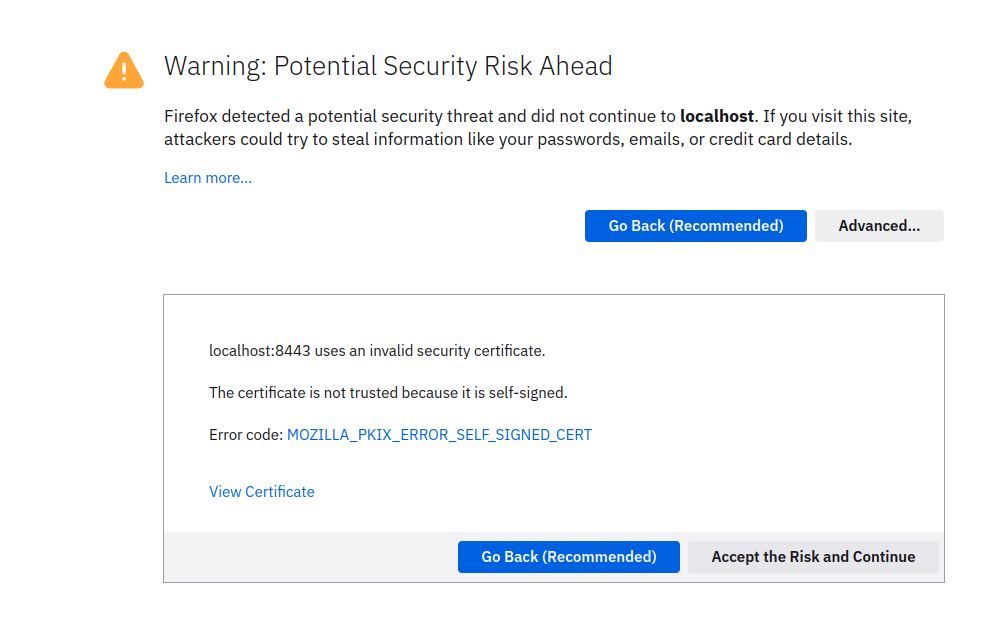
\includegraphics[width=\linewidth]{resources/firefox-warning.png}
    \end{subfigure}
    \begin{subfigure}[b]{0.3\linewidth}
        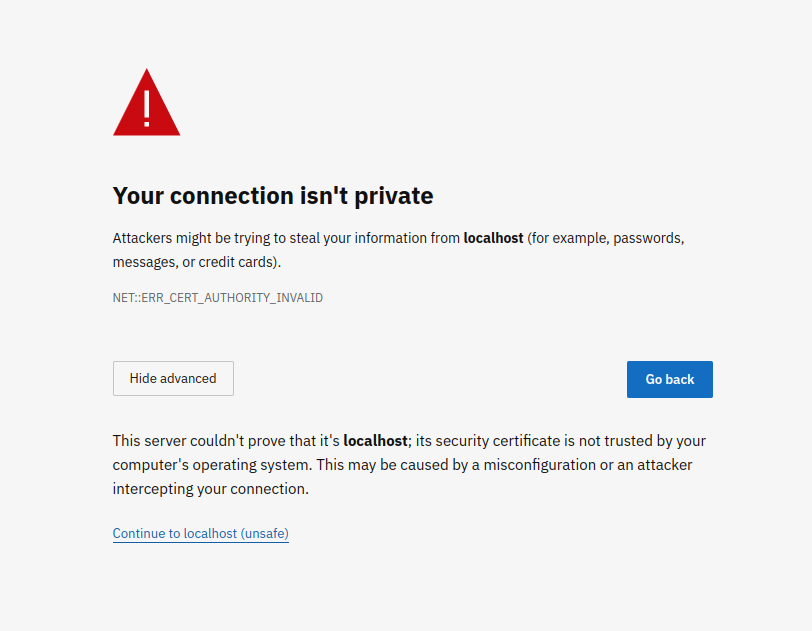
\includegraphics[width=\linewidth]{resources/edge-warning.png}
    \end{subfigure}
    \caption{Avviso presentato da diversi browser (Firefox a sinistra; Microsoft Edge a destra).}
\end{figure}

\section{Utilizzo}

\subsection{Generale}

\subsubsection{Registrazione}

\begin{figure}[H]
    \centering
    \begin{subfigure}[b]{0.4\linewidth}
        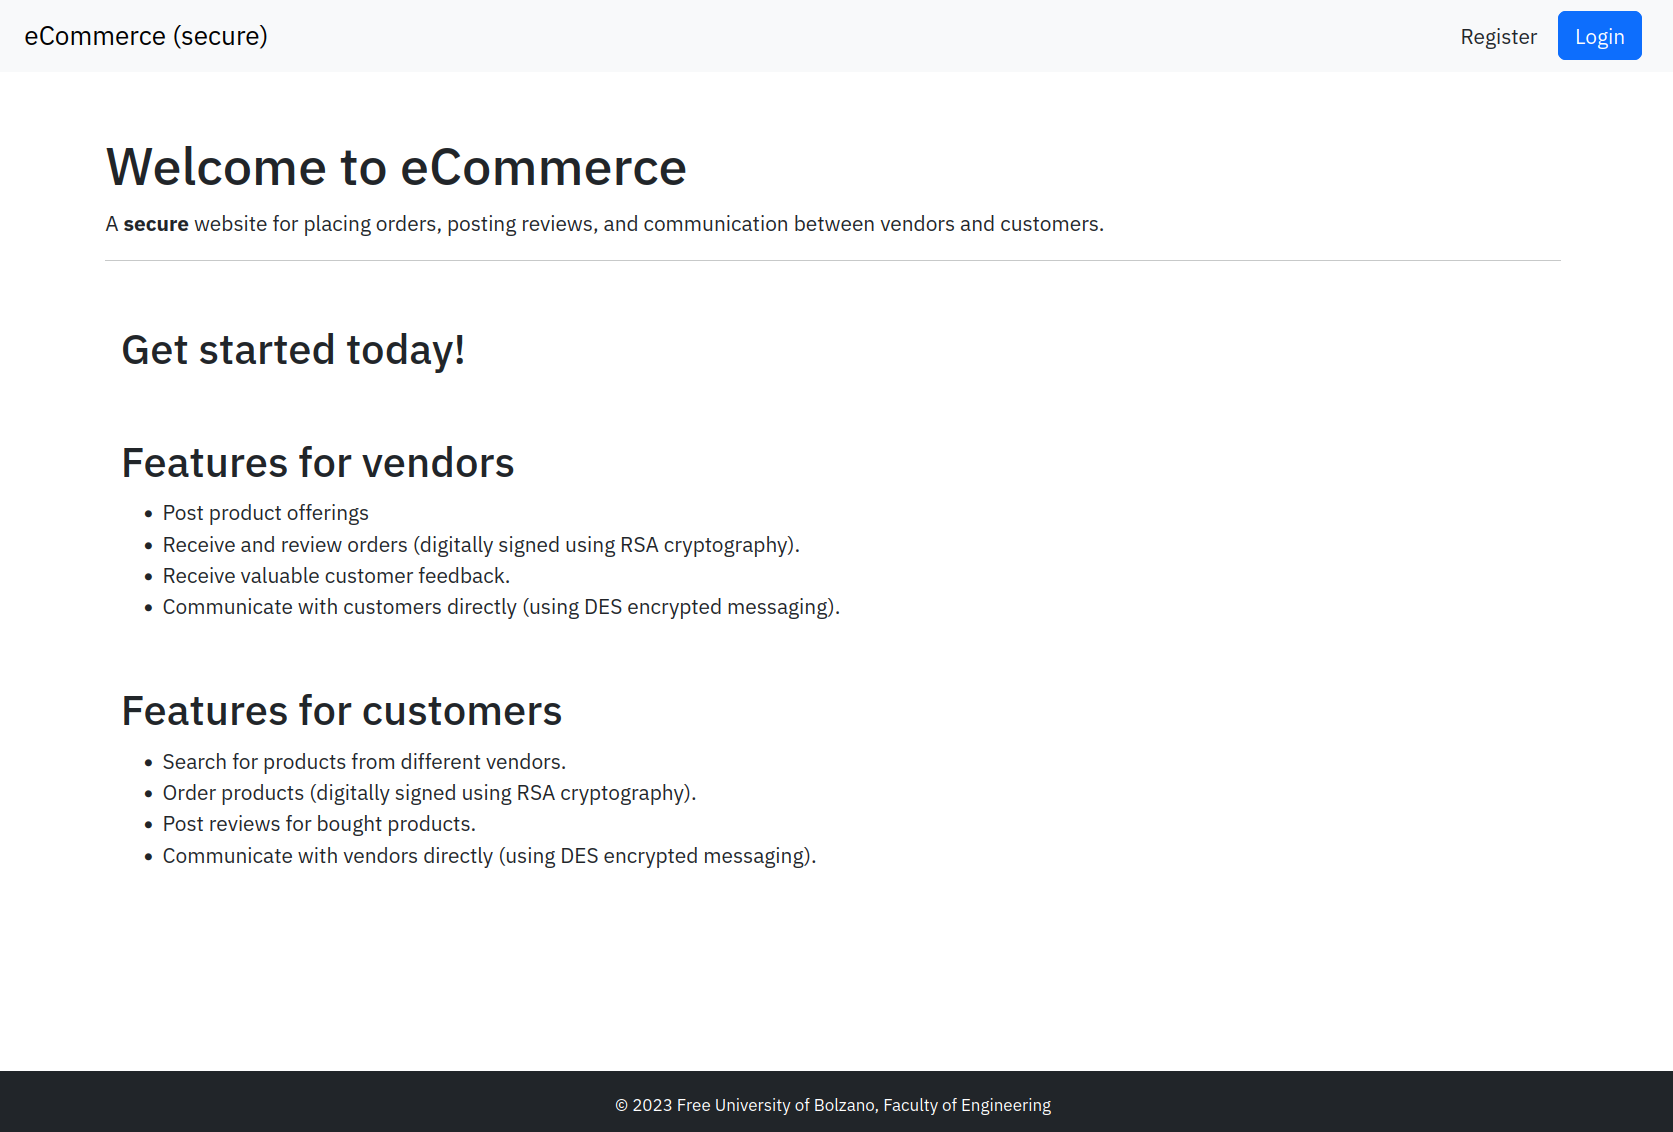
\includegraphics[width=\linewidth]{resources/welcome.png}
        \caption{La prima schermata presentata agli utenti.}
    \end{subfigure}
    \begin{subfigure}[b]{0.4\linewidth}
        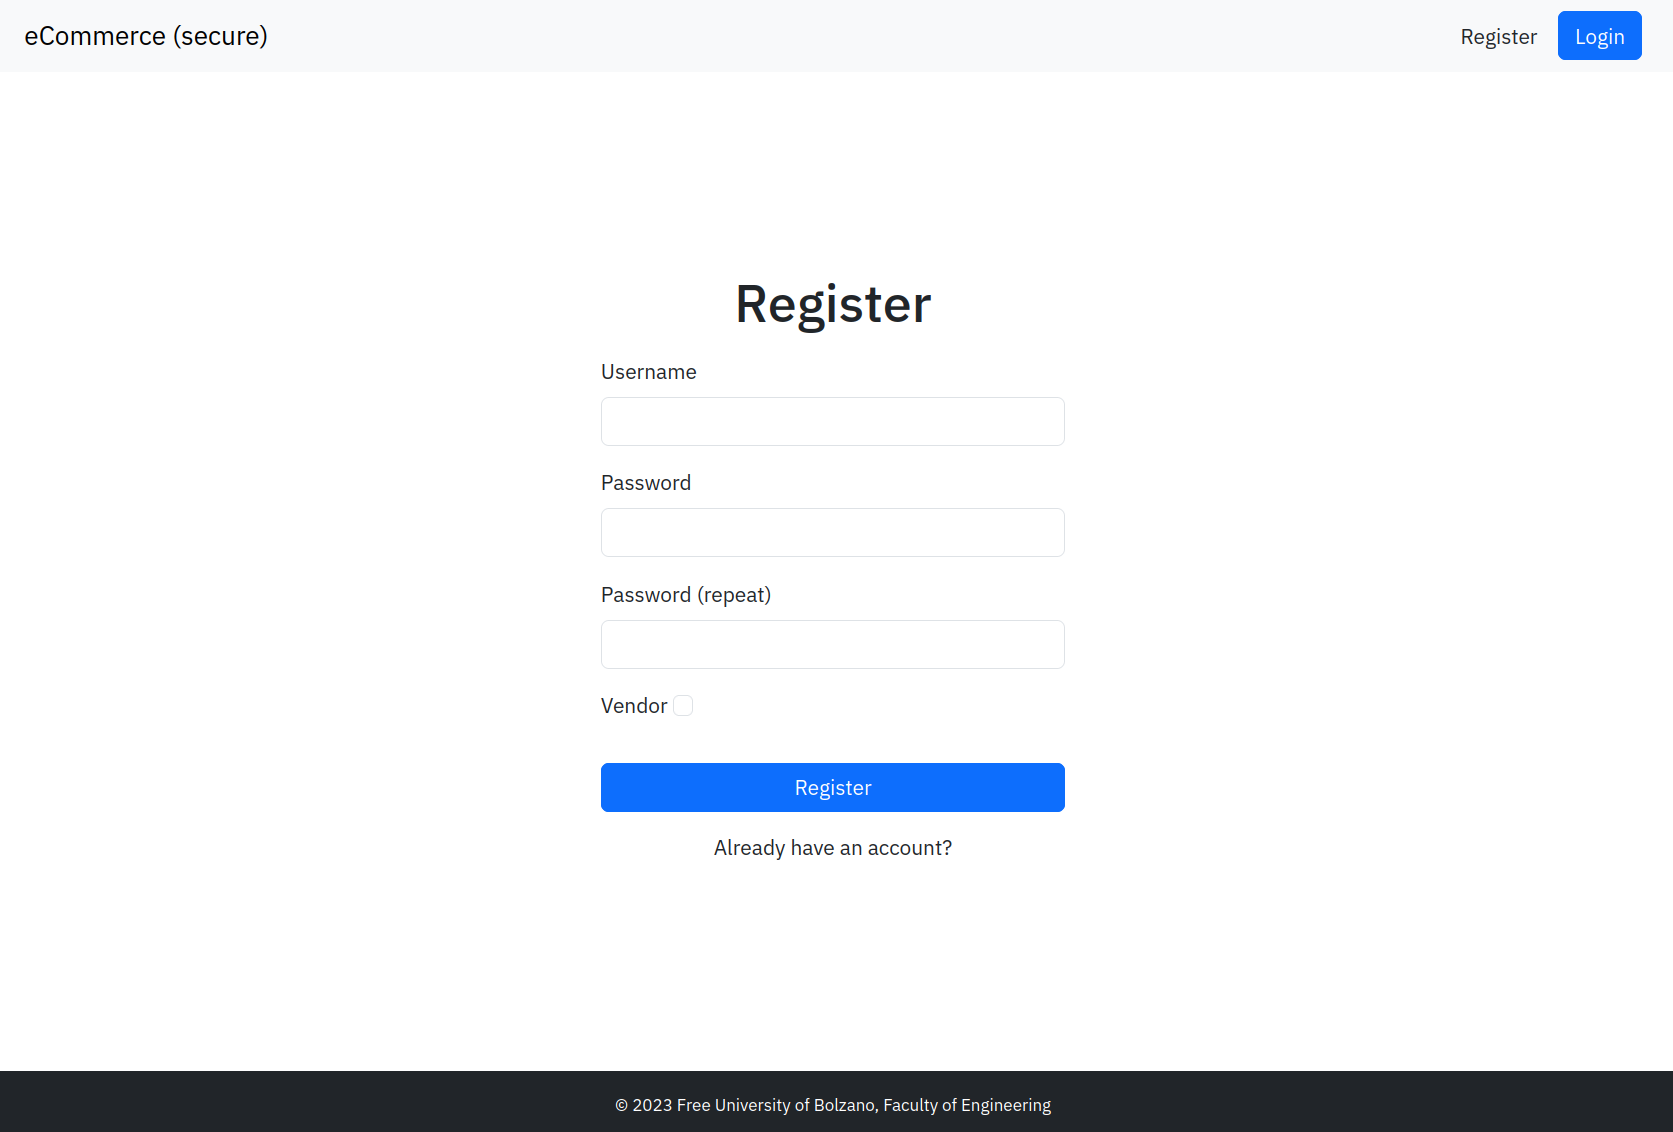
\includegraphics[width=\linewidth]{resources/register.png}
        \caption{Esempio di modulo di registrazione.}
    \end{subfigure}
    \caption{Esempio di procedura di registrazione.}
\end{figure}

Per registrarsi, l'utente deve fornire un nome utente contenente almeno 3 caratteri. Nella versione sicura, a parte i trattini bassi e i punti, i nomi utente possono contenere solo caratteri alfanumerici ASCII. All'utente viene inoltre chiesto di inserire una password due volte. Le due ripetizioni della password devono corrispondere e, nella versione sicura, ci sono ulteriori vincoli sulla password. Le password nella versione sicura devono essere lunghe almeno 8 caratteri, contenere lettere minuscole e maiuscole, numeri e caratteri speciali. I nomi utente sono unici, quindi se un altro utente ha già scelto il nome utente desiderato, la registrazione fallirà.

All'utente viene inoltre chiesto di dichiarare se è un venditore o un cliente. I venditori devono selezionare la casella di controllo in fondo al modulo con la dicitura "Vendor". I clienti e i venditori hanno accesso a funzionalità diverse e la scelta fatta durante la registrazione non può essere modificata in seguito.

\subsubsection{Login}

\begin{figure}[H]
    \centering
    \begin{subfigure}[b]{0.4\linewidth}
        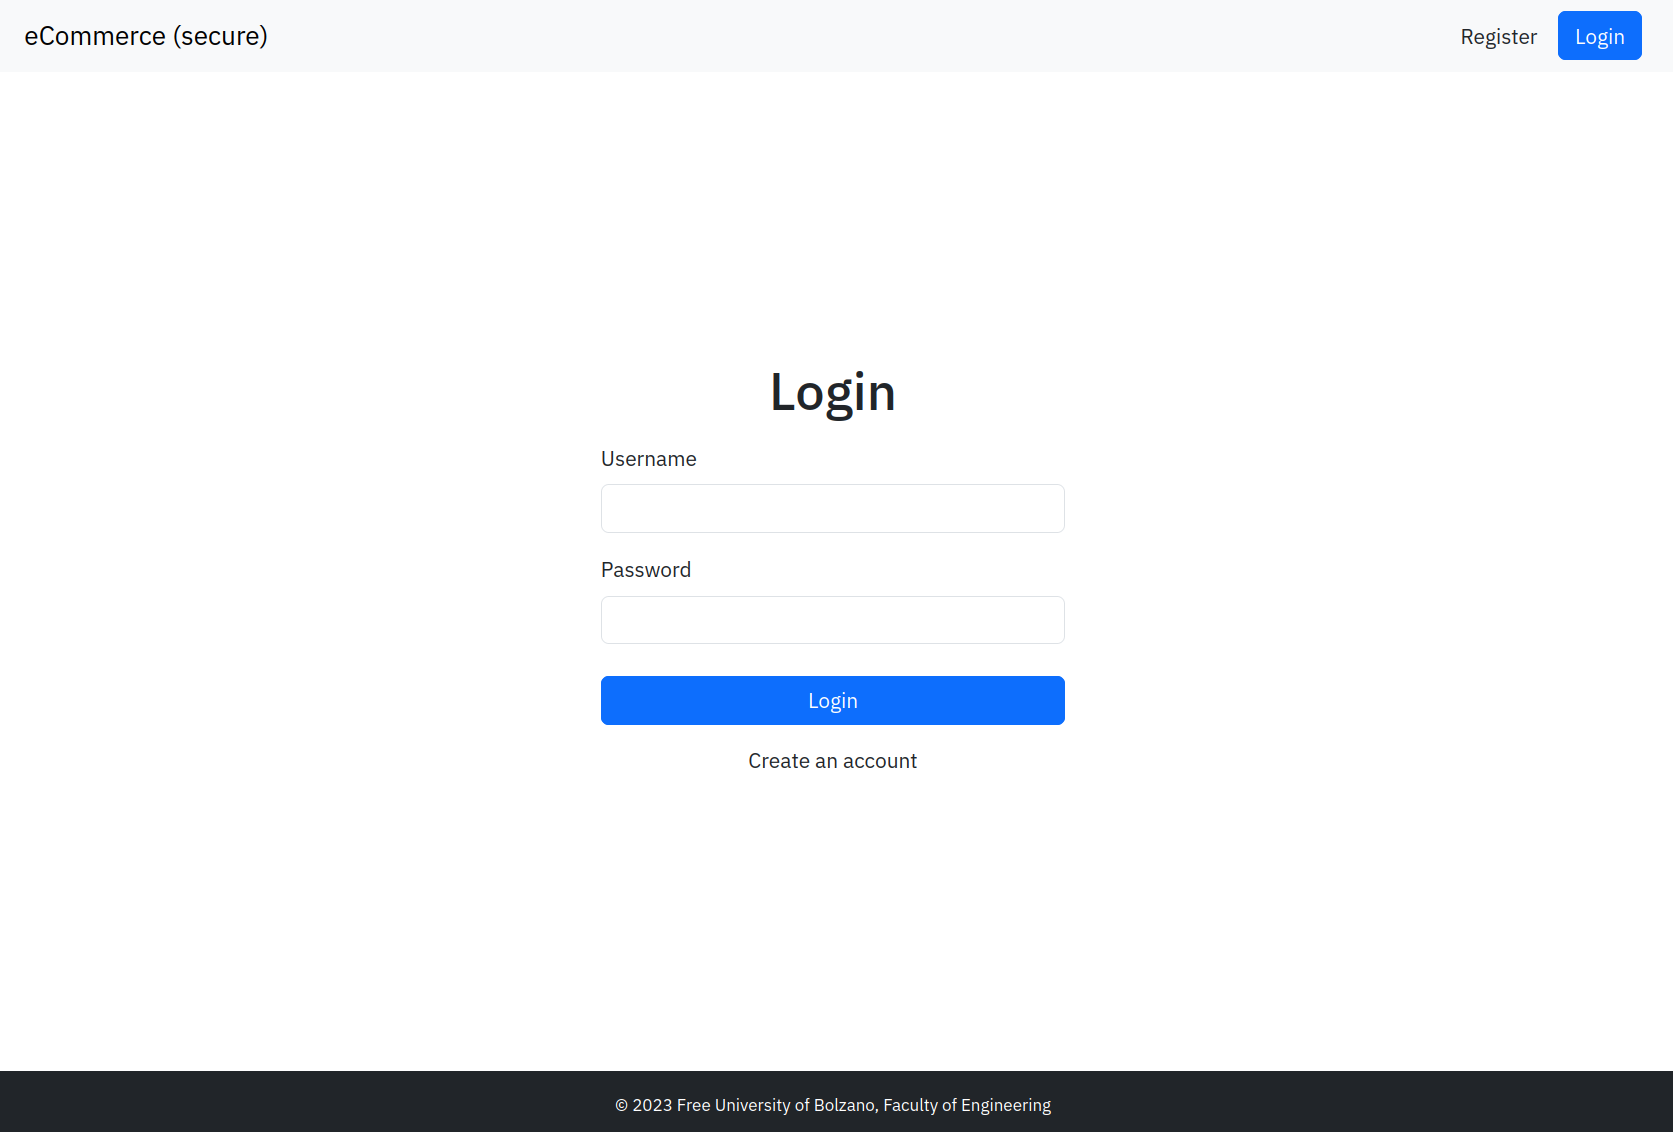
\includegraphics[width=\linewidth]{resources/login.png}
    \end{subfigure}
    \caption{Esempio di modulo di accesso.}
\end{figure}

Se l'utente ha già un account, può selezionare il pulsante "Already have an account?" o utilizzare il pulsante "Login" nell'intestazione del sito web. Per accedere all'applicazione web, l'utente deve fornire nome utente e password. Se questi non corrispondono a quelli di un utente noto, l'utente non potrà accedere a nessun'altra parte dell'applicazione.

\subsubsection{Ricerca e lettura dei prodotti}

\begin{figure}[H]
    \centering
    \begin{subfigure}[b]{0.4\linewidth}
        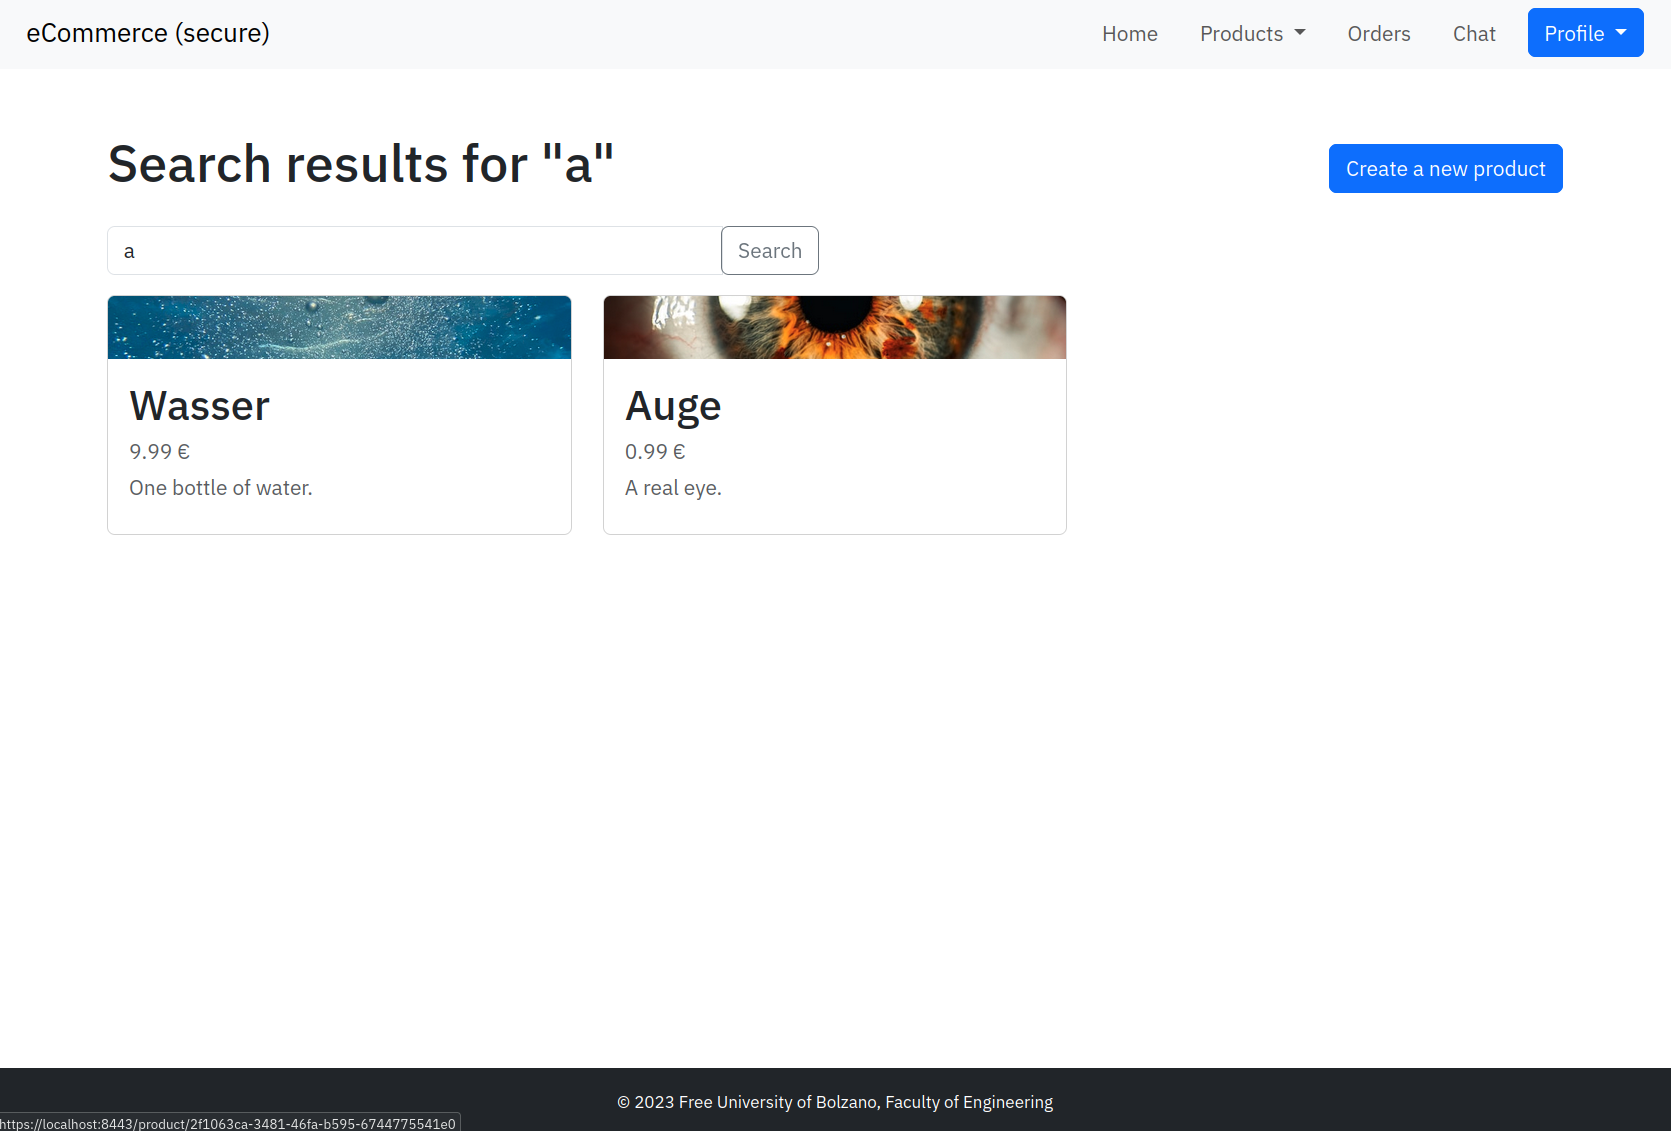
\includegraphics[width=\linewidth]{resources/seach-product.png}
        \caption{L'elenco di tutti i prodotti contenuti nella ricerca.}
    \end{subfigure}
    \begin{subfigure}[b]{0.4\linewidth}
        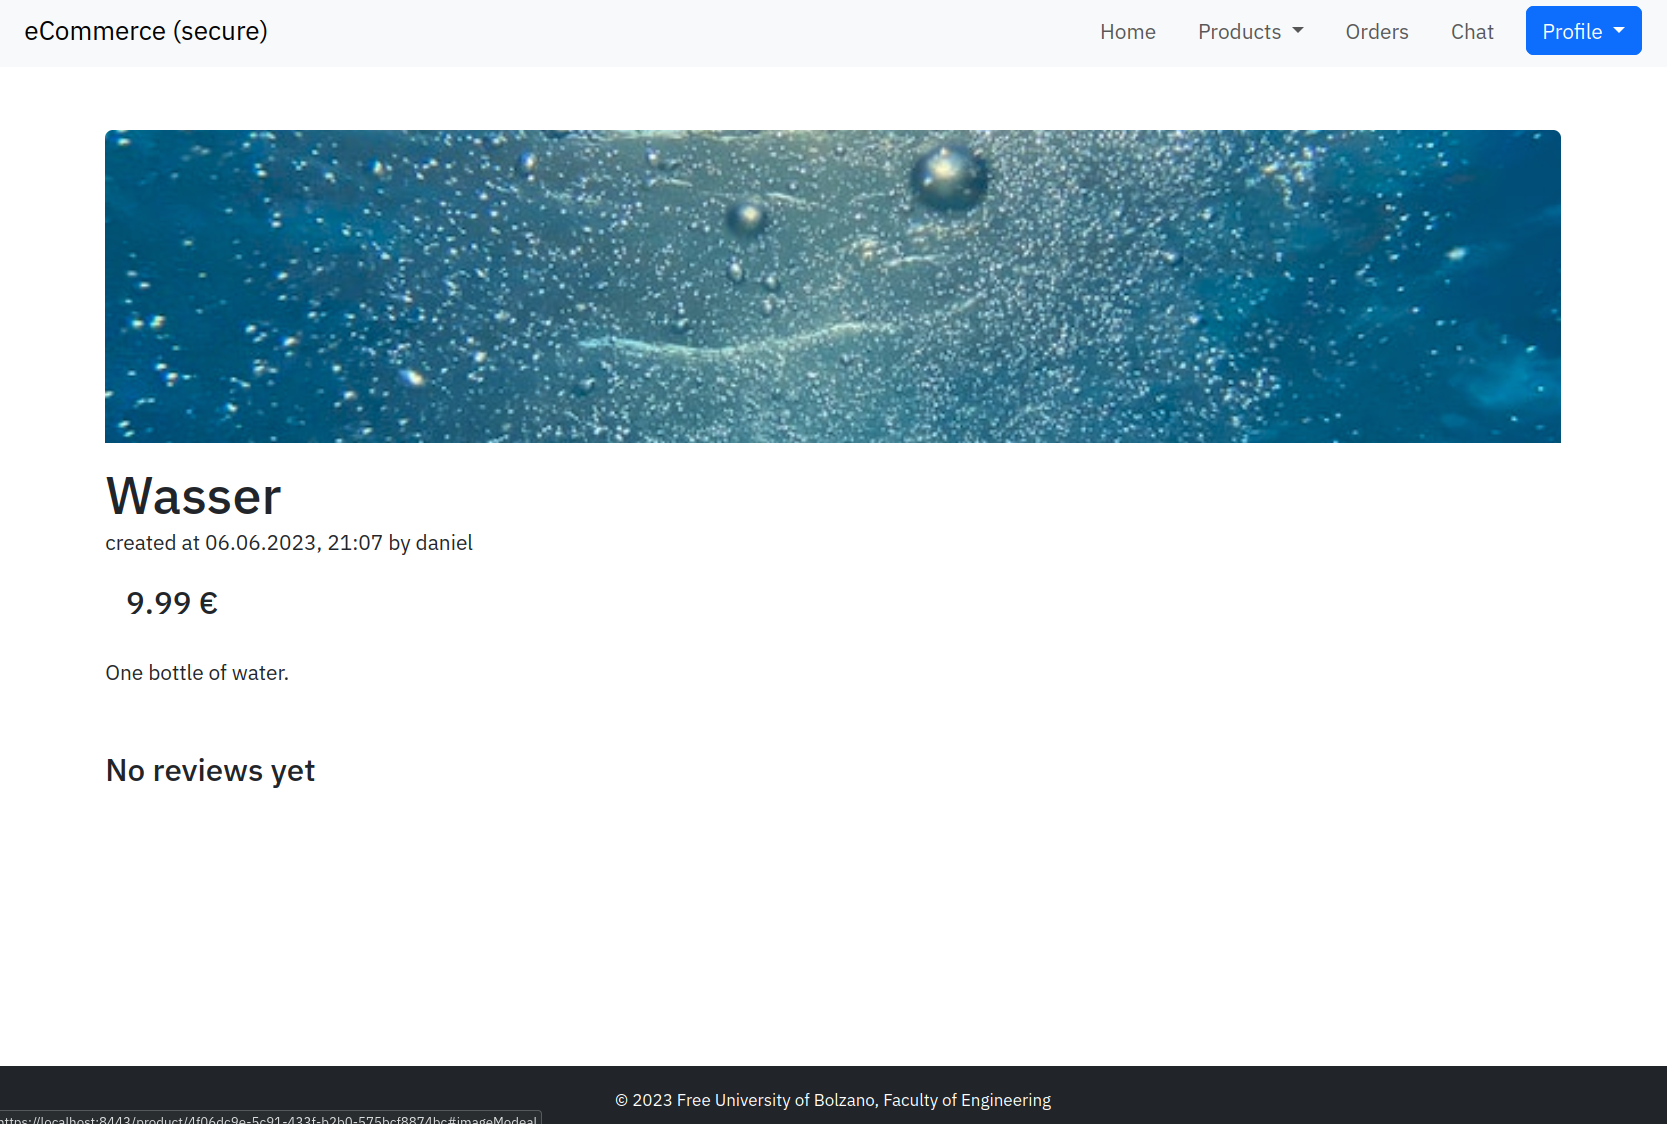
\includegraphics[width=\linewidth]{resources/product.png}
        \caption{Vista dettagliata di un prodotto.}
    \end{subfigure}
    \caption{Mostra il processo di ricerca e lettura delle schede prodotto.}
\end{figure}

Per cercare un prodotto, utilizzare il campo di ricerca all'inizio dell'elenco dei prodotti. L'elenco dei prodotti è accessibile tramite il menu "Products" nell'intestazione della pagina web. I venditori hanno a disposizione una versione speciale dell'elenco dei prodotti che mostra solo le schede dei prodotti da loro pubblicate sotto la voce di menu "My products". Per visualizzare ulteriori dettagli su un singolo prodotto, selezionarlo nell'elenco dei prodotti facendo clic sulla scheda del prodotto. Questa è anche la sezione in cui sono visibili le recensioni dei prodotti e le risposte a tali recensioni.

\subsection{Venditori}

\subsubsection{Pubblicare un prodotto}

\begin{figure}[H]
    \centering
    \begin{subfigure}[b]{0.4\linewidth}
        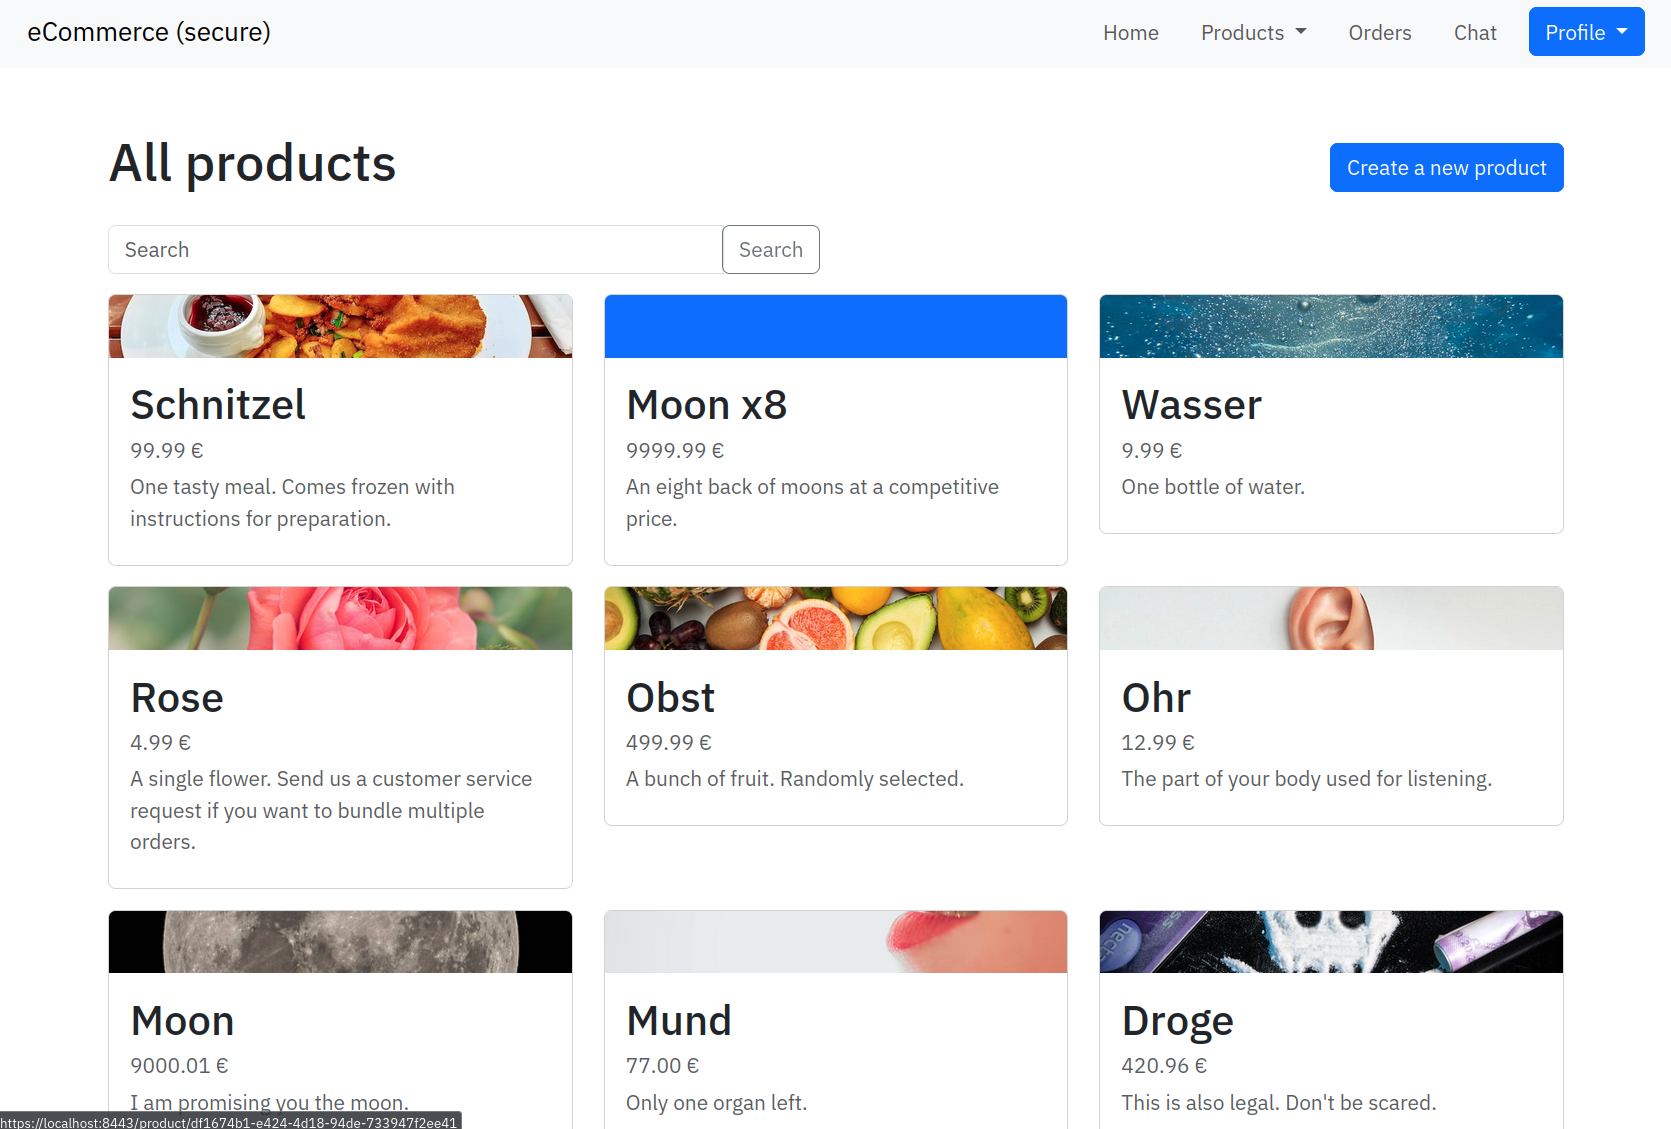
\includegraphics[width=\linewidth]{resources/products.png}
        \caption{L'elenco di tutti i prodotti attualmente pubblicati.}
    \end{subfigure}
    \begin{subfigure}[b]{0.4\linewidth}
        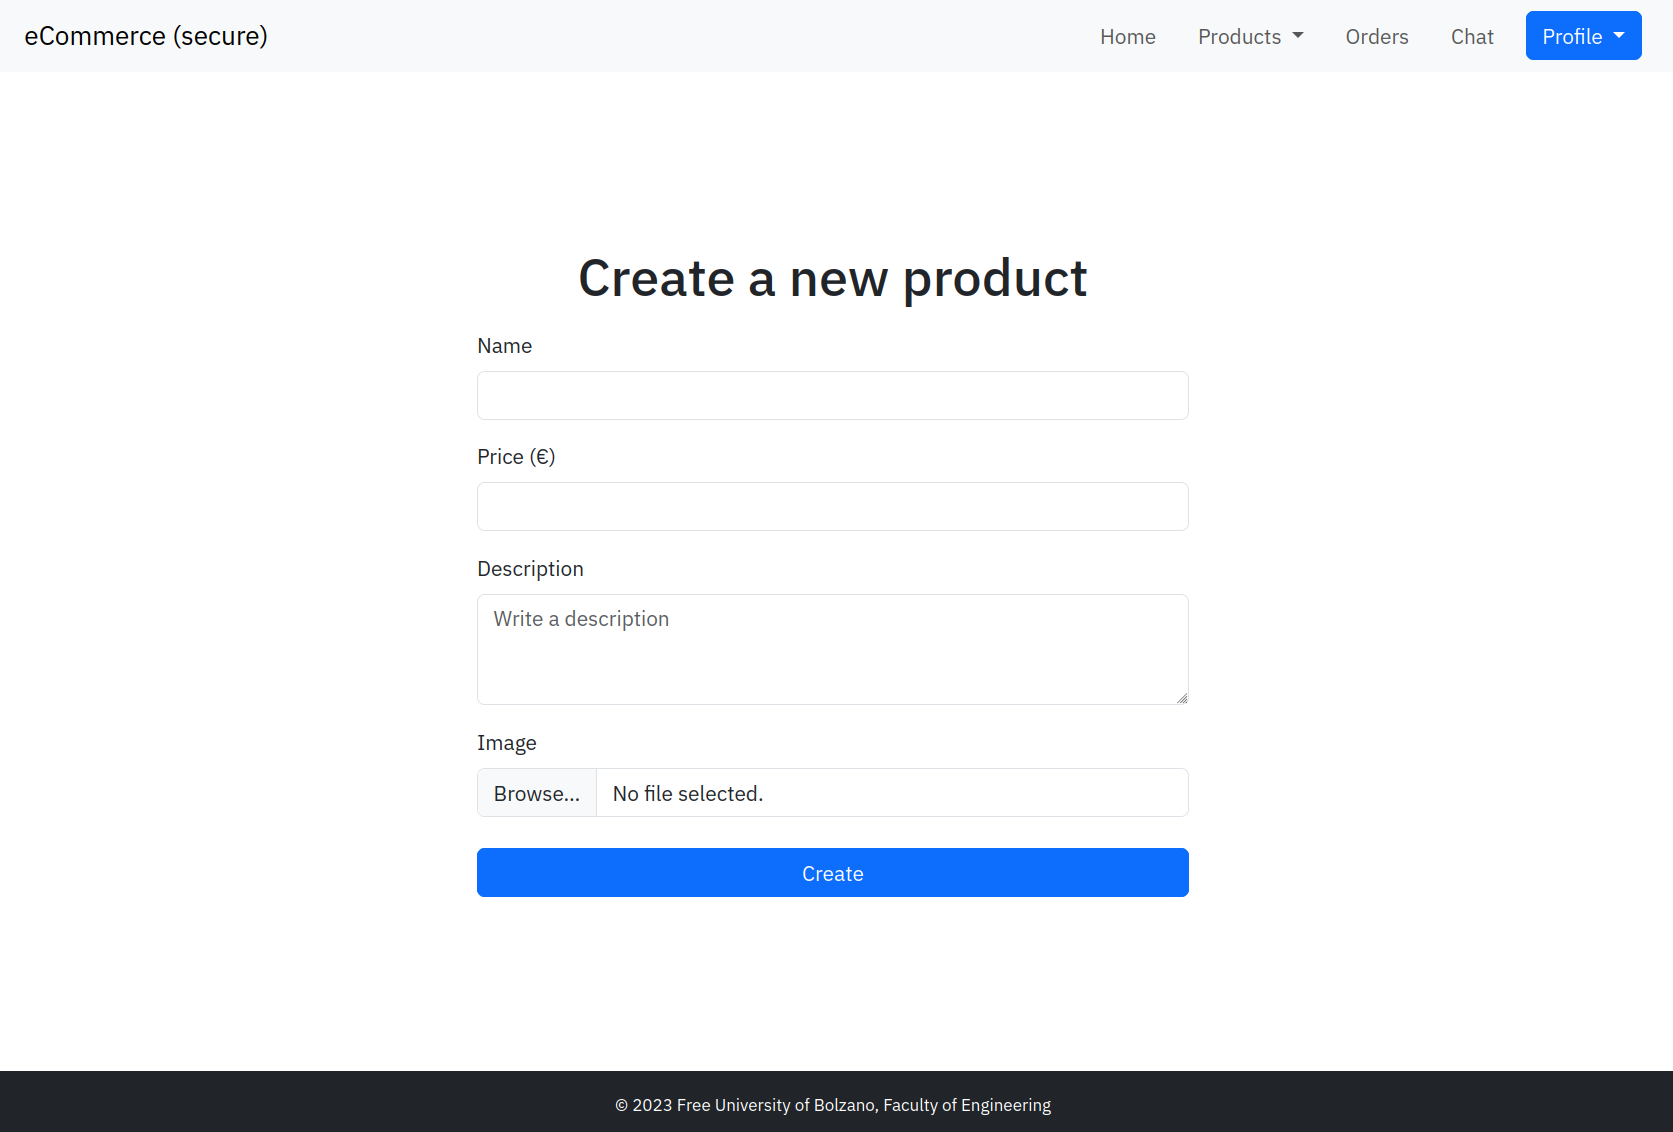
\includegraphics[width=\linewidth]{resources/new-product.png}
        \caption{Esempio di modulo per la creazione di nuovi post sui prodotti.}
    \end{subfigure}
    \caption{Esempio delle fasi di creazione di un nuovo prodotto.}
\end{figure}

I venditori possono inserire nuovi prodotti navigando in uno degli elenchi di prodotti attraverso il menu "Products" nell'intestazione della pagina web e selezionando "Create a new product". All'utente verrà presentato un modulo che richiede il nome del prodotto, il prezzo, la descrizione e l'immagine. Il nome del prodotto e il prezzo sono obbligatori, mentre la descrizione e l'immagine possono essere lasciate facoltativamente vuote.

\subsubsection{Controlla gli ordini}

\begin{figure}[H]
    \centering
    \begin{subfigure}[b]{0.4\linewidth}
        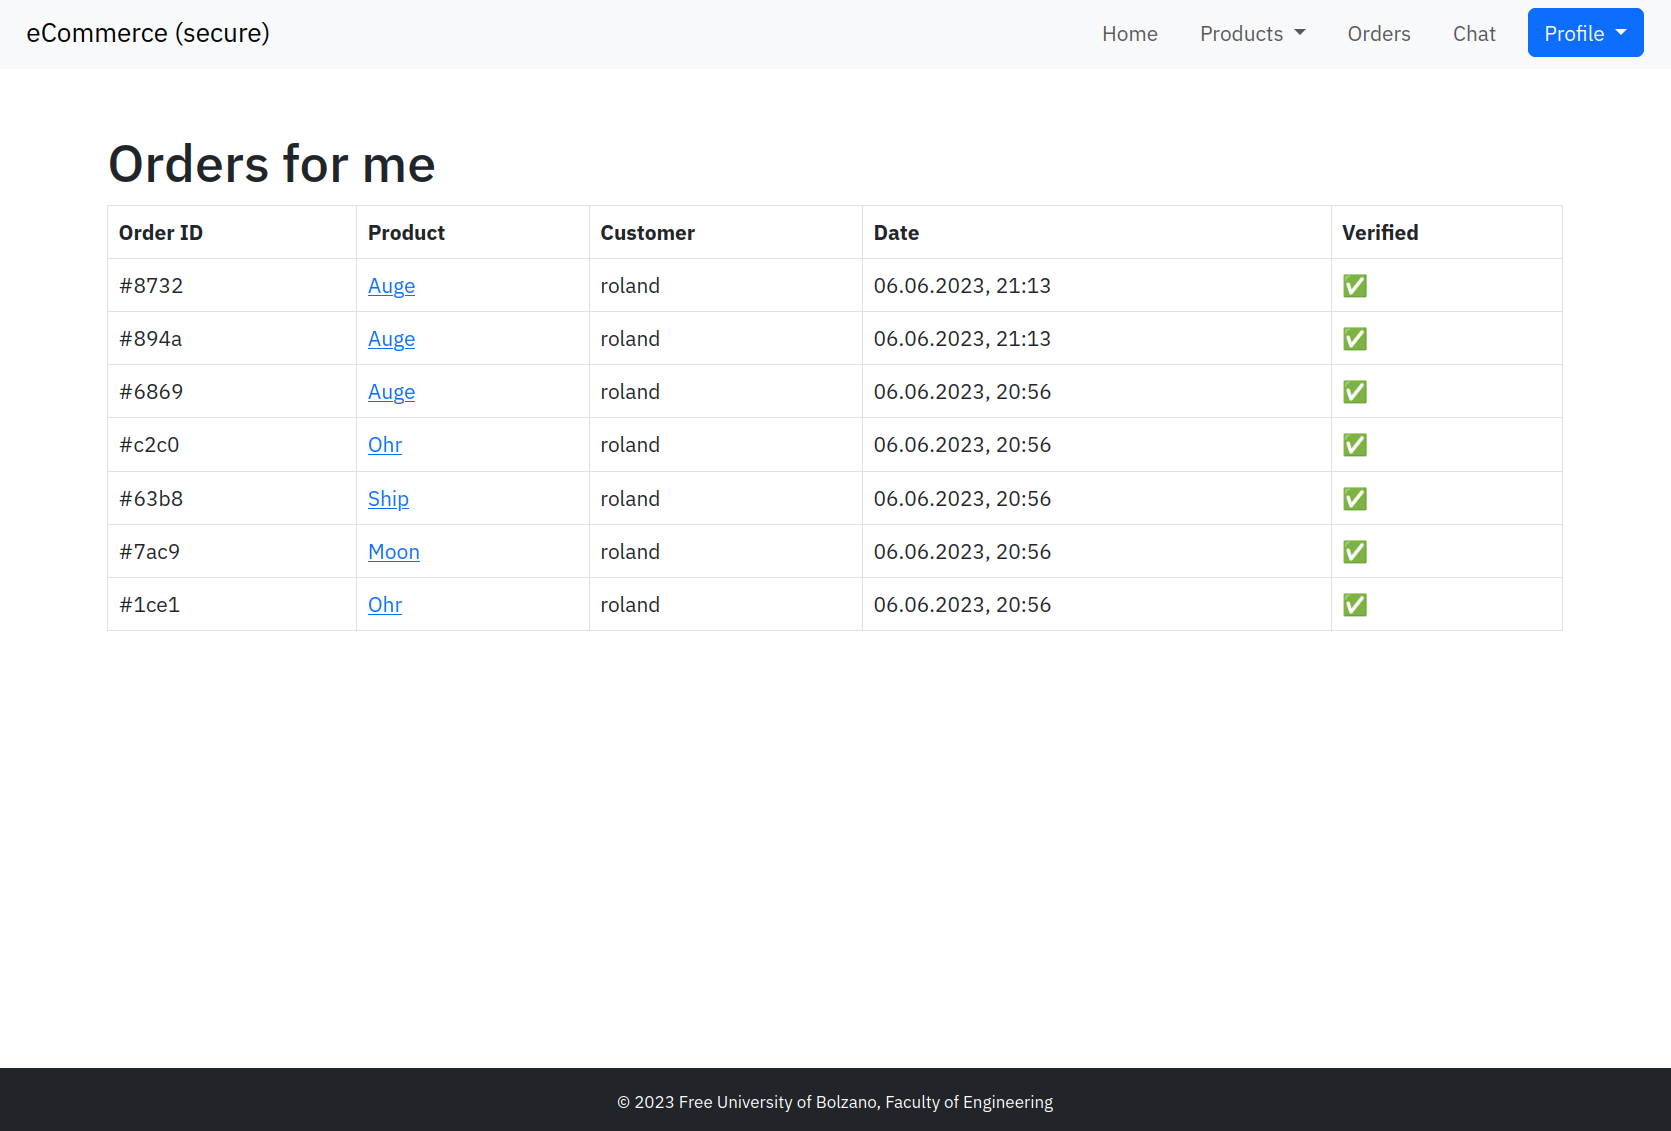
\includegraphics[width=\linewidth]{resources/orders.png}
    \end{subfigure}
    \caption{Esempio che mostra l'elenco degli ordini per i prodotti di un fornitore.}
\end{figure}

Un venditore può controllare gli ordini in arrivo dai suoi clienti navigando nella vista ordini utilizzando il pulsante "Orders" della barra di navigazione superiore. Per ogni ordine vengono visualizzati l'identificativo dell'ordine, il prodotto acquistato, il cliente che ha effettuato l'acquisto e i dati dell'acquisto. Inoltre, la versione sicura dell'applicazione supporta anche la firma digitale dei documenti dell'ordine. Se l'ordine ha una firma valida nel database, viene visualizzato un segno di spunta. Se la firma non è presente o è in qualche modo non valida, viene visualizzato un segno di spunta rosso per quell'ordine.

\subsubsection{Rispondi alle recensioni}

\begin{figure}[H]
    \centering
    \begin{subfigure}[b]{0.4\linewidth}
        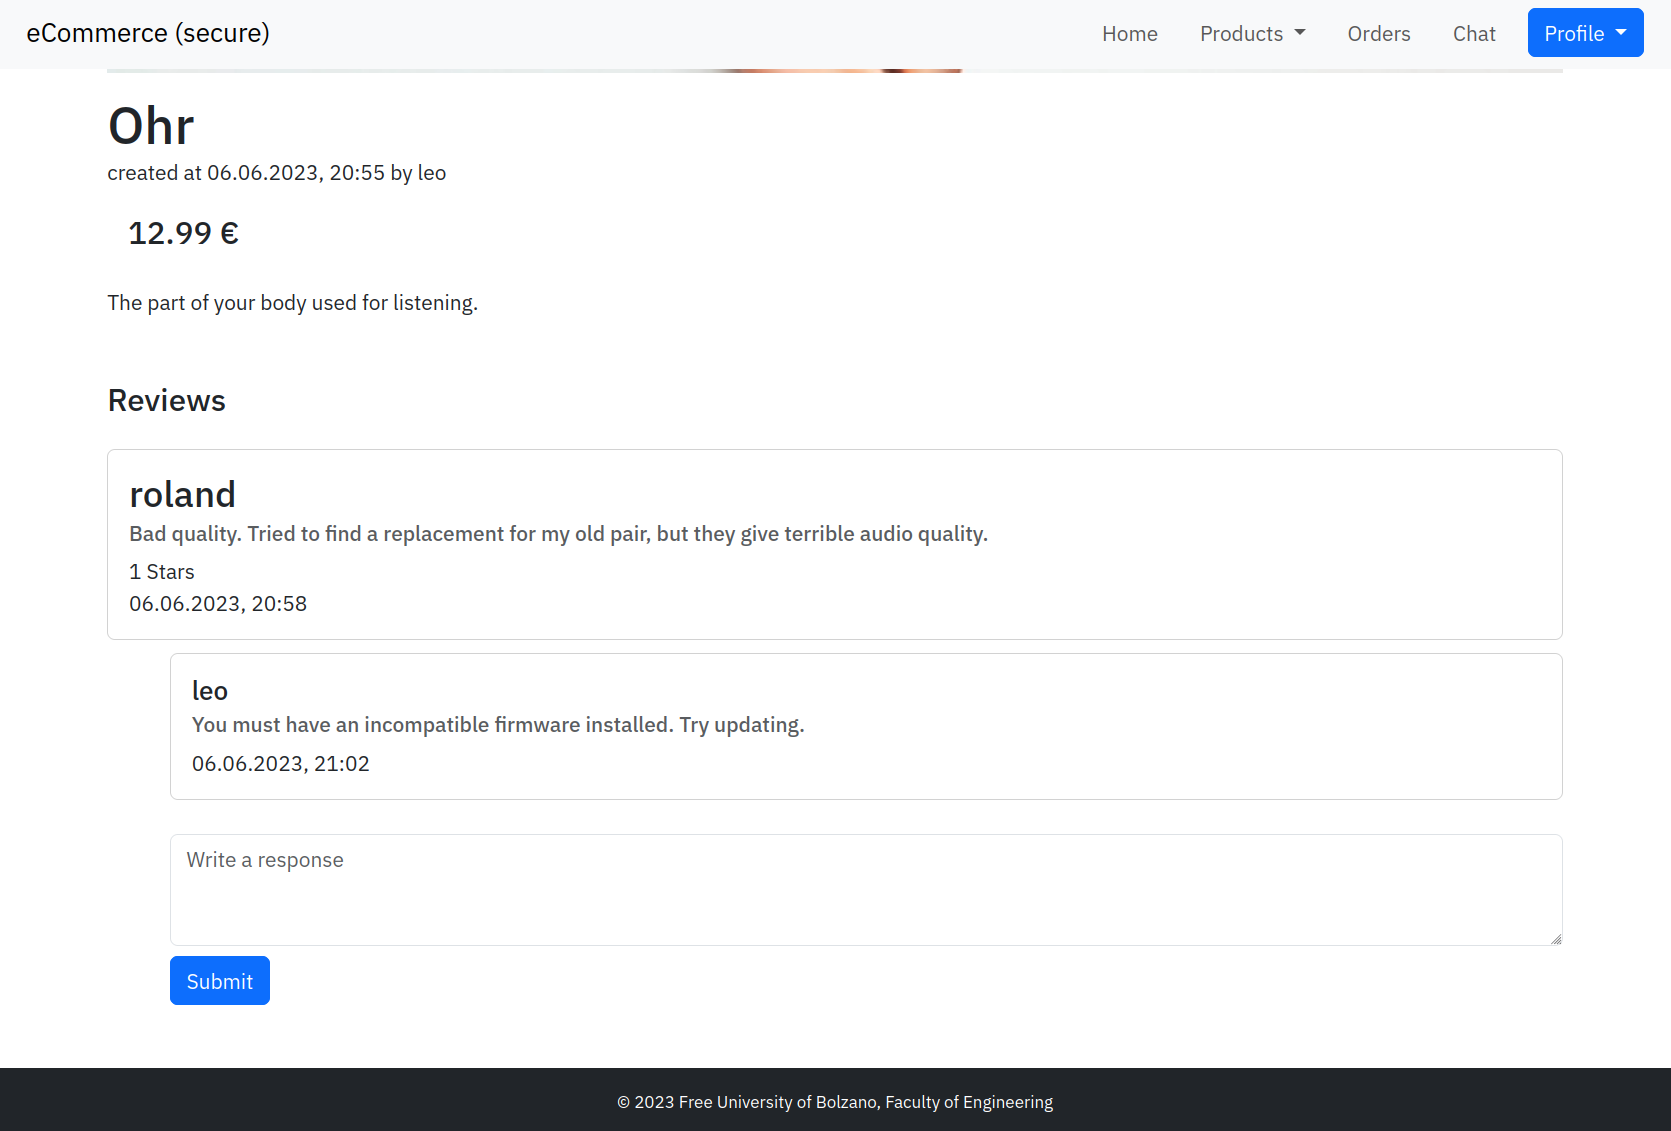
\includegraphics[width=\linewidth]{resources/response.png}
    \end{subfigure}
    \caption{Esempio di come i venditori possono rispondere alle recensioni.}
\end{figure}

Se un cliente ha pubblicato una recensione per un prodotto di un fornitore, quest'ultimo può rispondere alla recensione. Ciò è possibile navigando nella pagina delle informazioni sul prodotto e scrivendo la risposta nel campo di testo sotto la recensione. Per inviare la risposta, premere il pulsante "Submit" sotto l'area di testo.

\subsubsection{Chat con i clienti}

\begin{figure}[H]
    \centering
    \begin{subfigure}[b]{0.4\linewidth}
        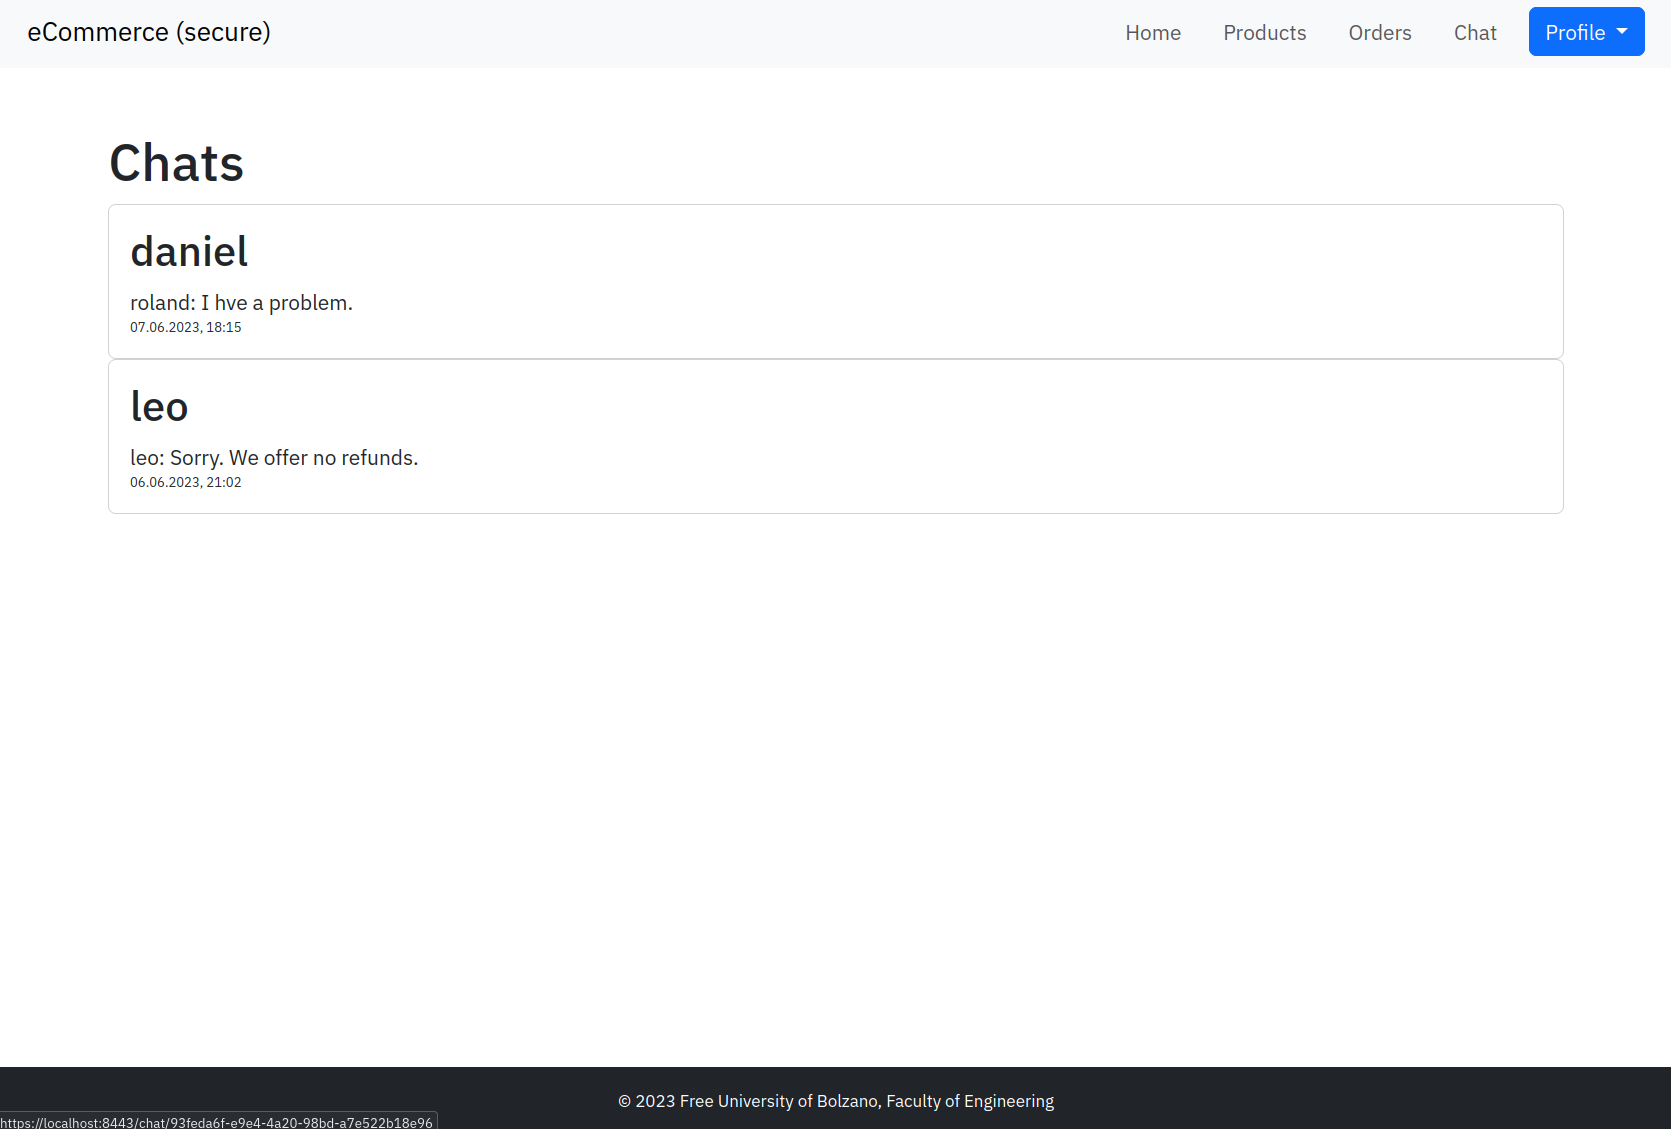
\includegraphics[width=\linewidth]{resources/chat-list.png}
        \caption{Elenco di tutti gli utenti con cui il fornitore ha comunicato.}
    \end{subfigure}
    \begin{subfigure}[b]{0.4\linewidth}
        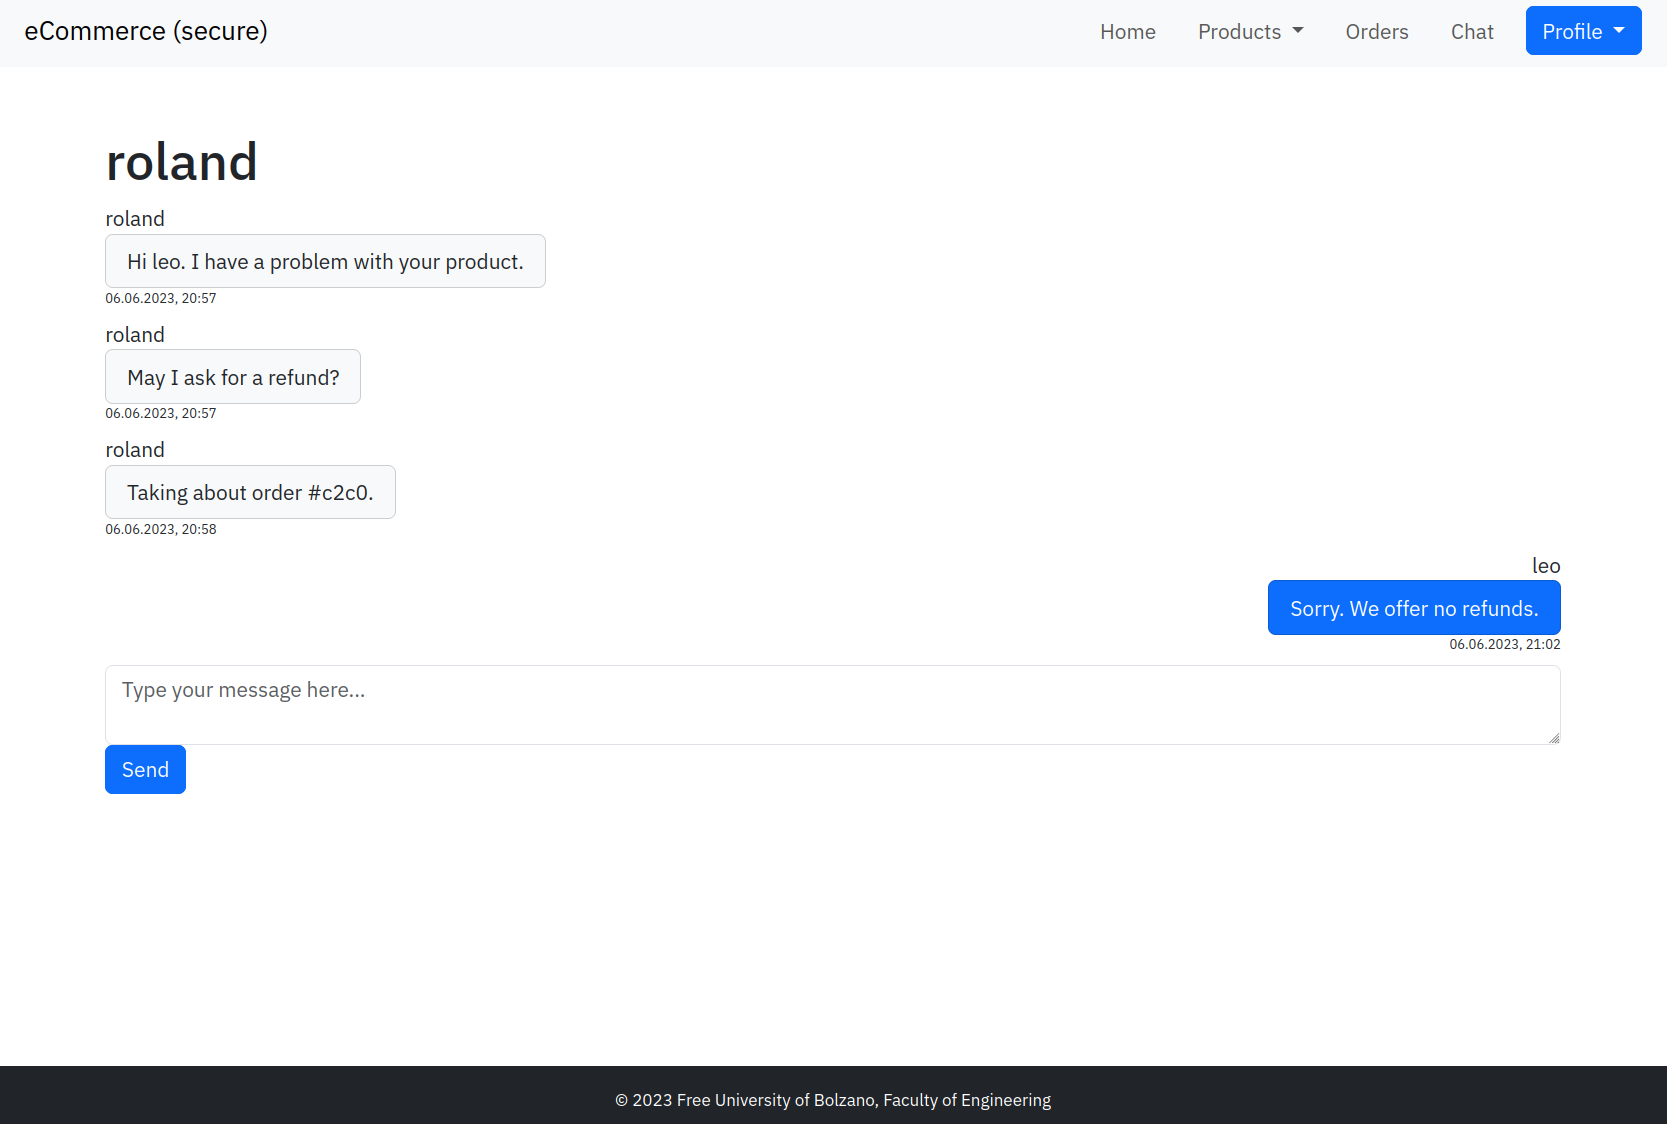
\includegraphics[width=\linewidth]{resources/chat.png}
        \caption{Un esempio di chat con un cliente.}
    \end{subfigure}
    \caption{Esempio di come i venditori possono chattare con i clienti.}
\end{figure}

L'applicazione offre ai clienti la possibilità di inviare messaggi ai venditori tramite una chat privata. Il venditore può vedere tutti gli utenti con cui ha scambiato messaggi di chat navigando nell'elenco delle chat utilizzando il pulsante "Chat" nel menu in cima alla pagina. Selezionando una delle chat, l'utente può digitare un messaggio nell'area di testo in fondo alla pagina e fare clic su "Submit" per inviarmi il messaggio. I messaggi sono memorizzati in modo criptato con l'algoritmo DES e non sono accessibili a nessuno, se non agli utenti che partecipano alla comunicazione.


\subsection{Clienti}

\subsubsection{Acquista prodotti}

\begin{figure}[H]
    \centering
    \begin{subfigure}[b]{0.4\linewidth}
        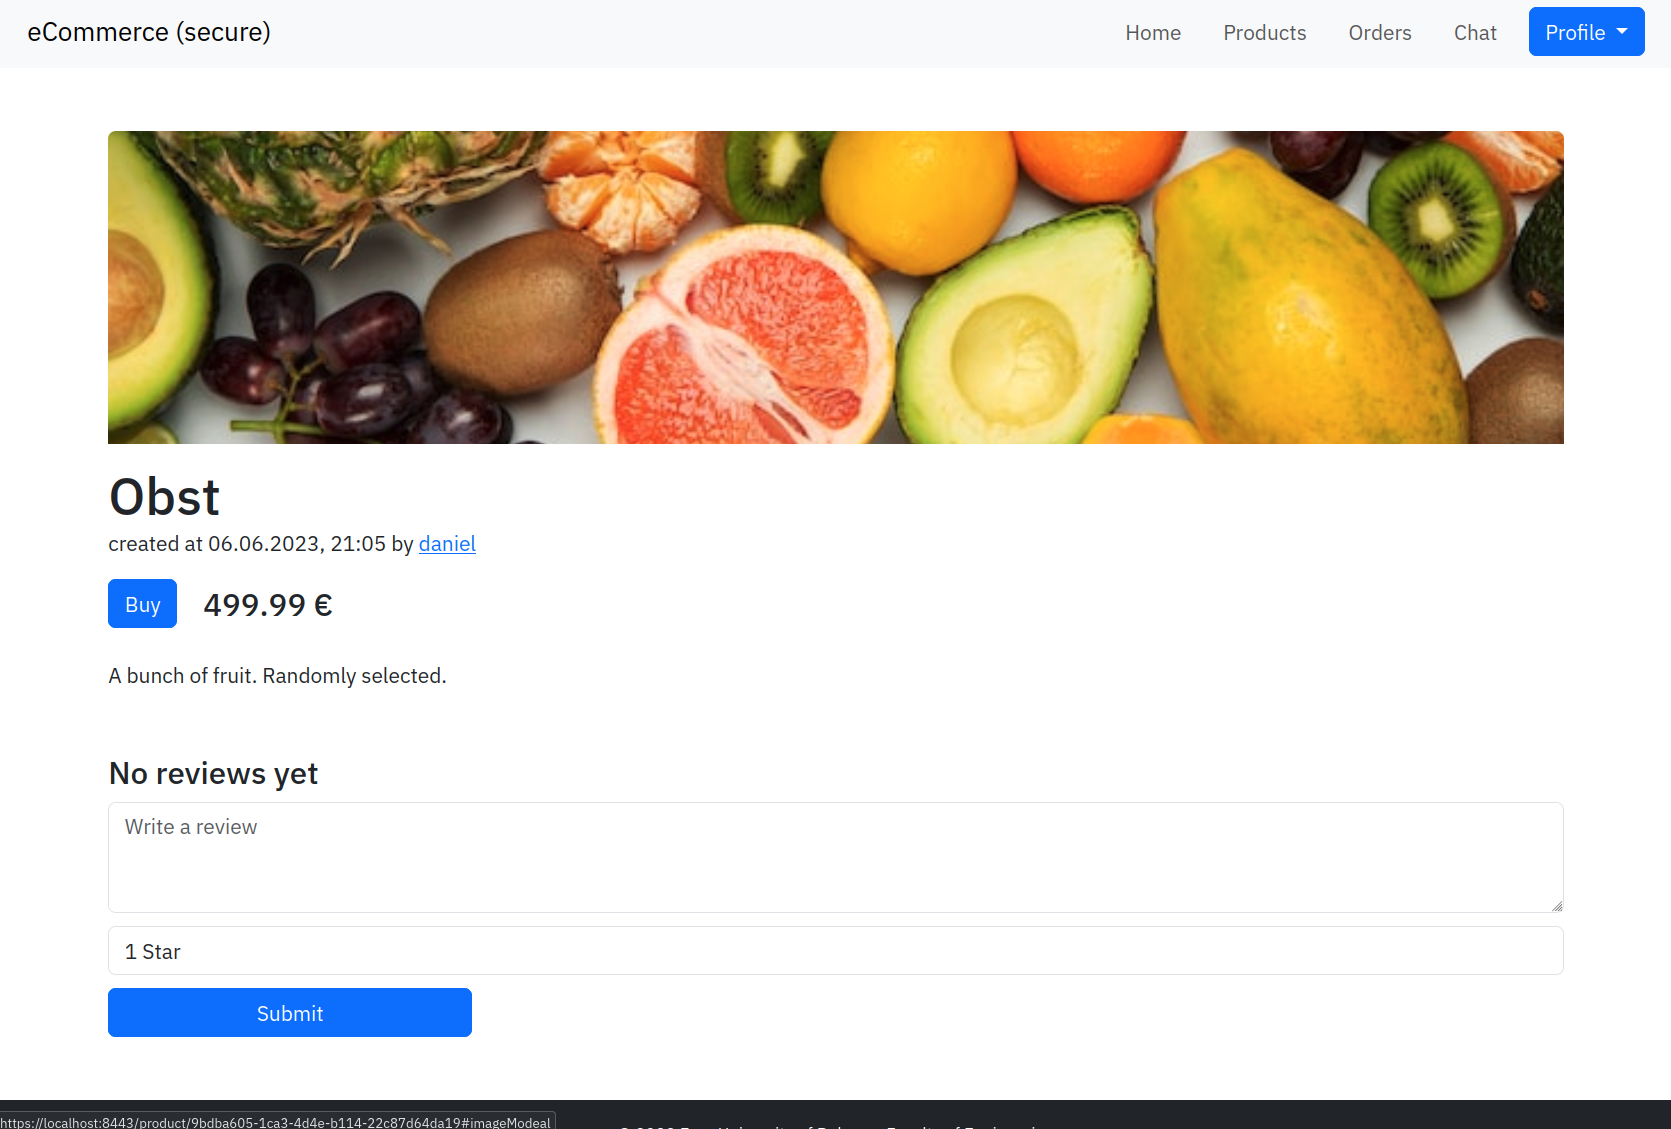
\includegraphics[width=\linewidth]{resources/product-customer.png}
        \caption{La pagina dei dettagli del prodotto per un cliente.}
    \end{subfigure}
    \begin{subfigure}[b]{0.4\linewidth}
        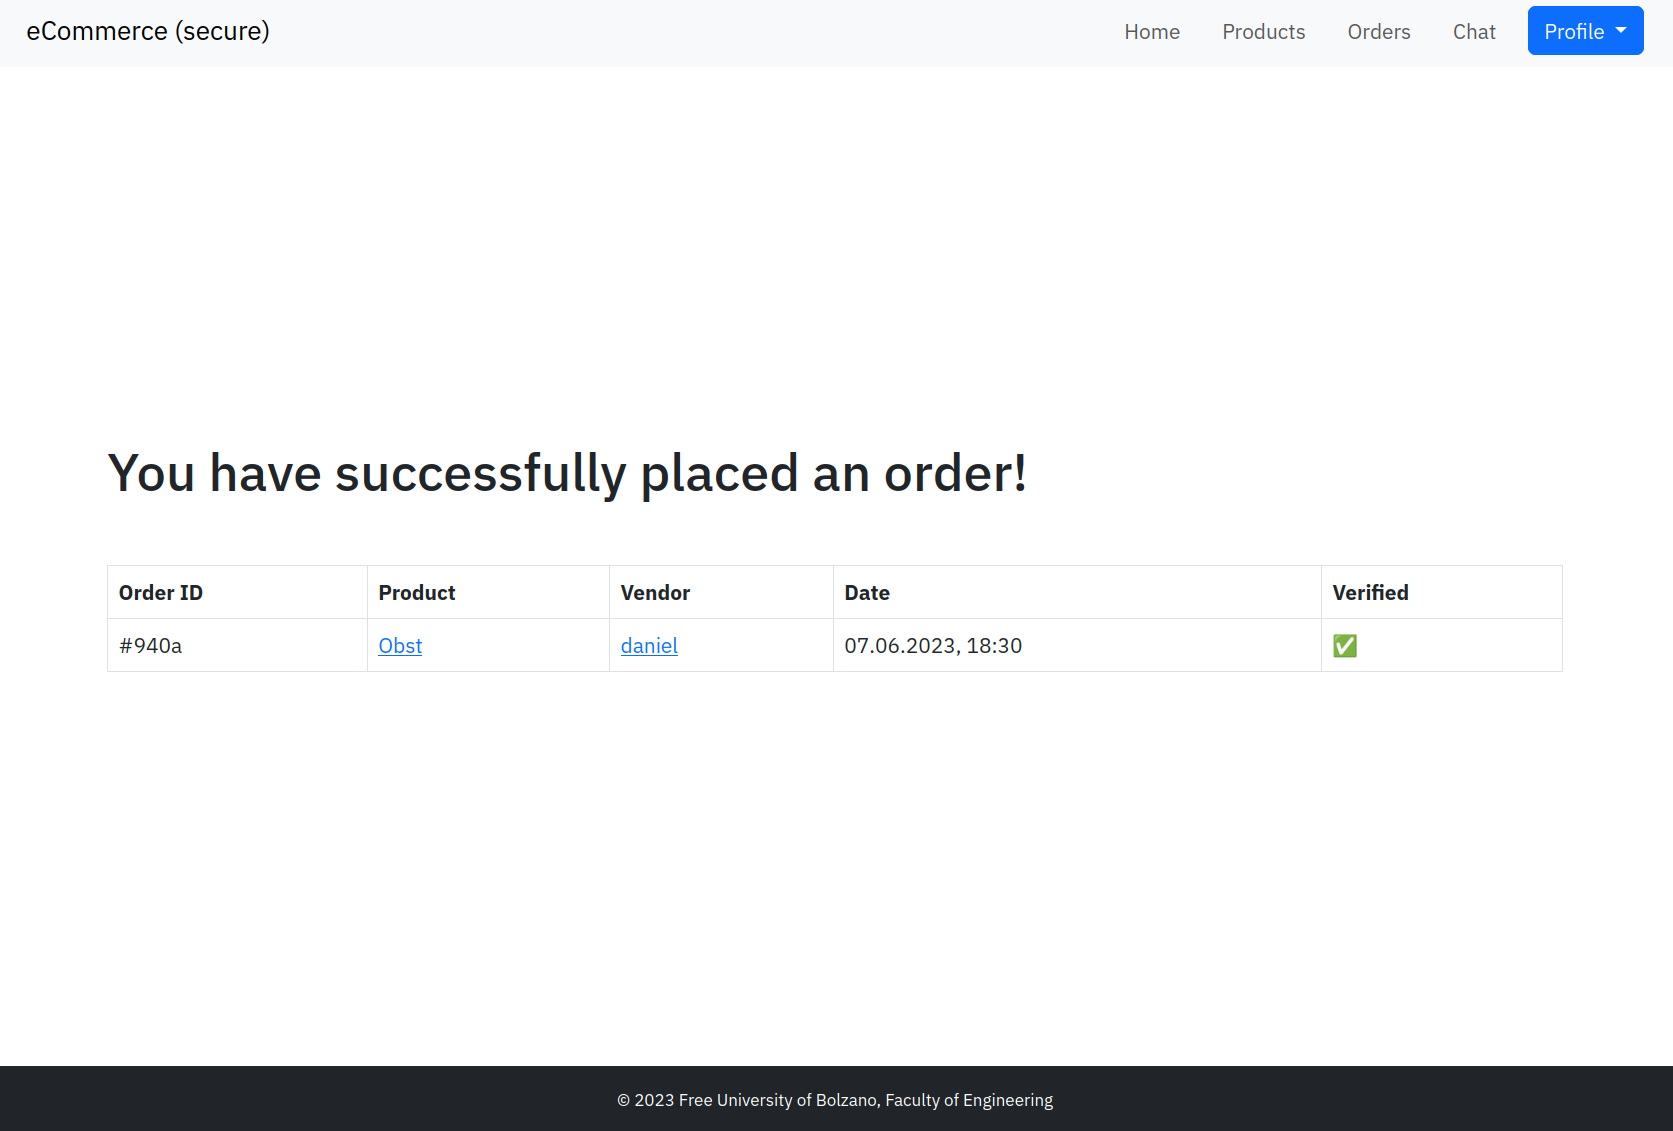
\includegraphics[width=\linewidth]{resources/order.png}
        \caption{Esempio di pagina visualizzata dopo aver effettuato un ordine.}
    \end{subfigure}
    \caption{Esempio di come un cliente può effettuare un ordine.}
\end{figure}

Per effettuare un ordine di un prodotto, il cliente può navigare nella pagina dei dettagli del prodotto. Da qui, il cliente può acquistare un prodotto utilizzando il pulsante "Buy" sopra la descrizione del prodotto. Dopo aver effettuato l'ordine, viene visualizzata una pagina di conferma che riporta anche le informazioni relative al documento d'ordine e, per la versione sicura, se è stato firmato con successo con una firma digitale.

\subsubsection{Pubblica una recensione}

\begin{figure}[H]
    \centering
    \begin{subfigure}[b]{0.4\linewidth}
        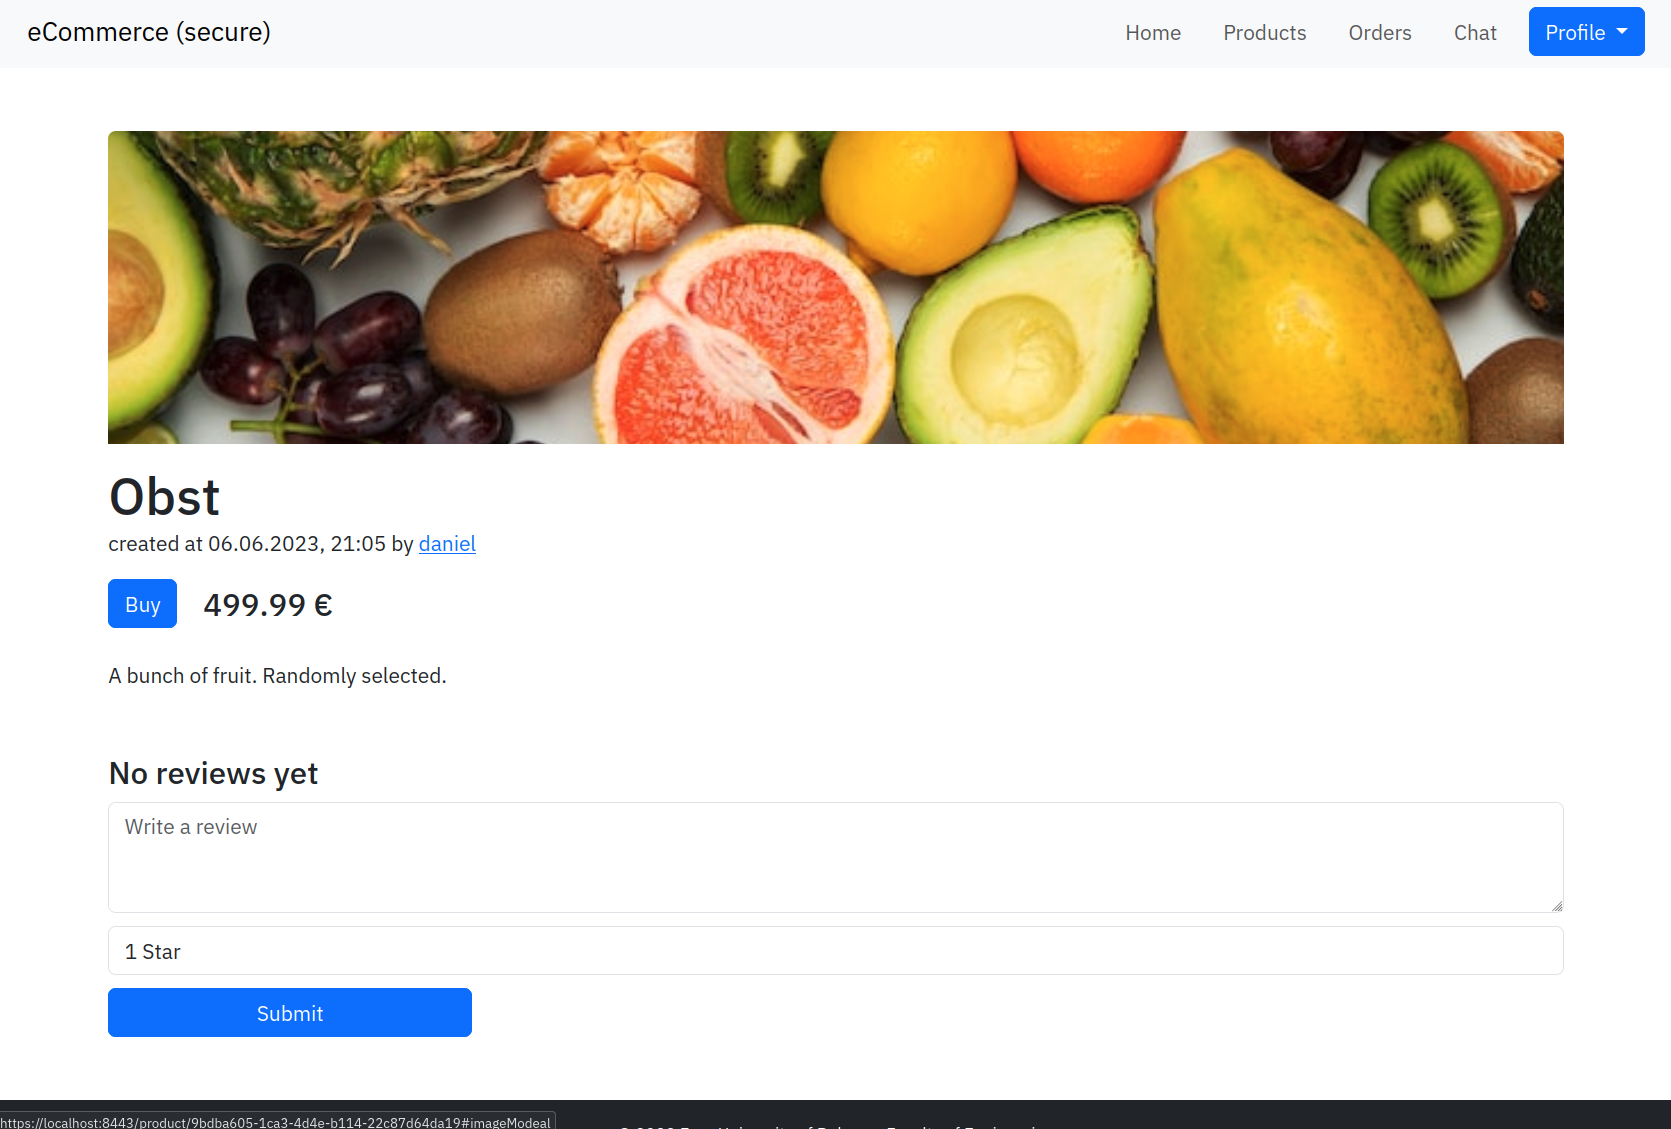
\includegraphics[width=\linewidth]{resources/product-customer.png}
    \end{subfigure}
    \caption{Esempio di pagina di prodotto in cui gli utenti possono pubblicare recensioni.}
\end{figure}

Dopo che l'utente ha acquistato un prodotto, la pagina dei dettagli del prodotto mostrerà l'opzione di pubblicare una recensione. Utilizzando l'area di testo all'inizio dell'elenco delle recensioni, selezionando una valutazione iniziale da 1 a 5 e facendo clic sul pulsante "Submit", è possibile pubblicare una recensione.

\subsubsection{Chat con i venditori}

\begin{figure}[H]
    \centering
    \begin{subfigure}[b]{0.4\linewidth}
        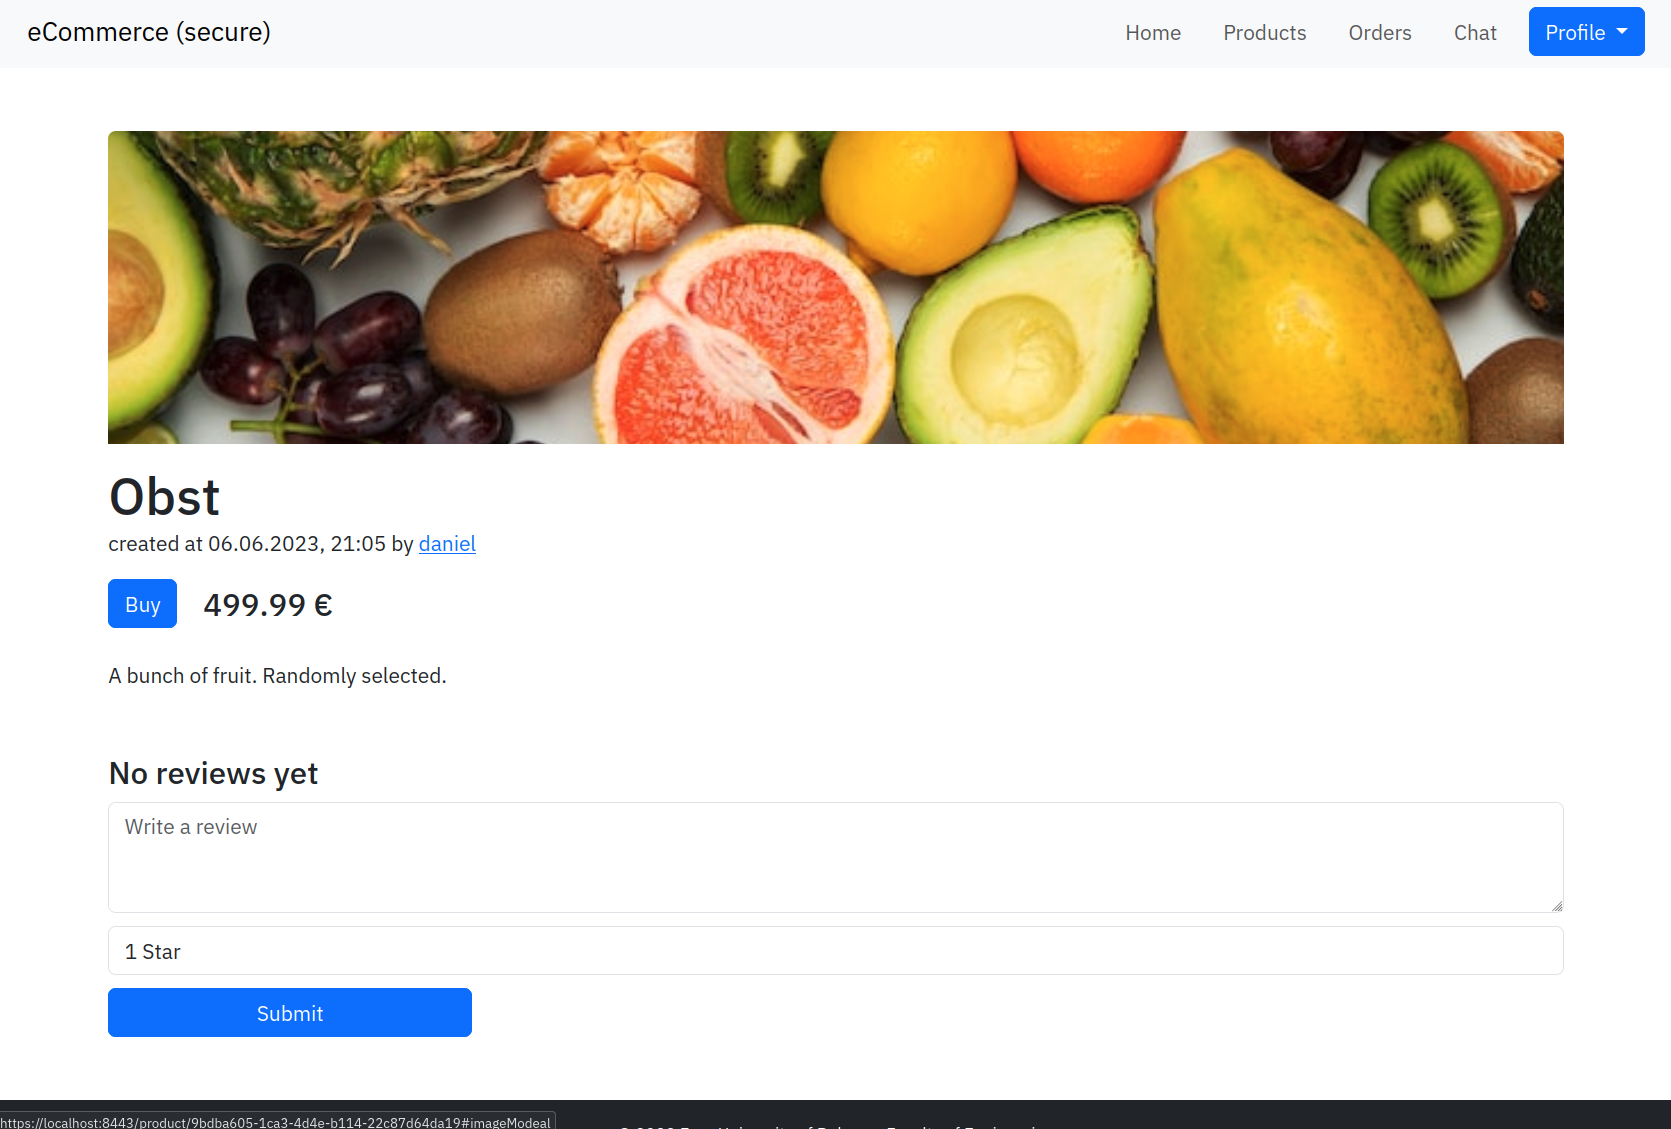
\includegraphics[width=\linewidth]{resources/product-customer.png}
        \caption{La pagina dei dettagli del prodotto per un cliente.}
    \end{subfigure}
    \begin{subfigure}[b]{0.4\linewidth}
        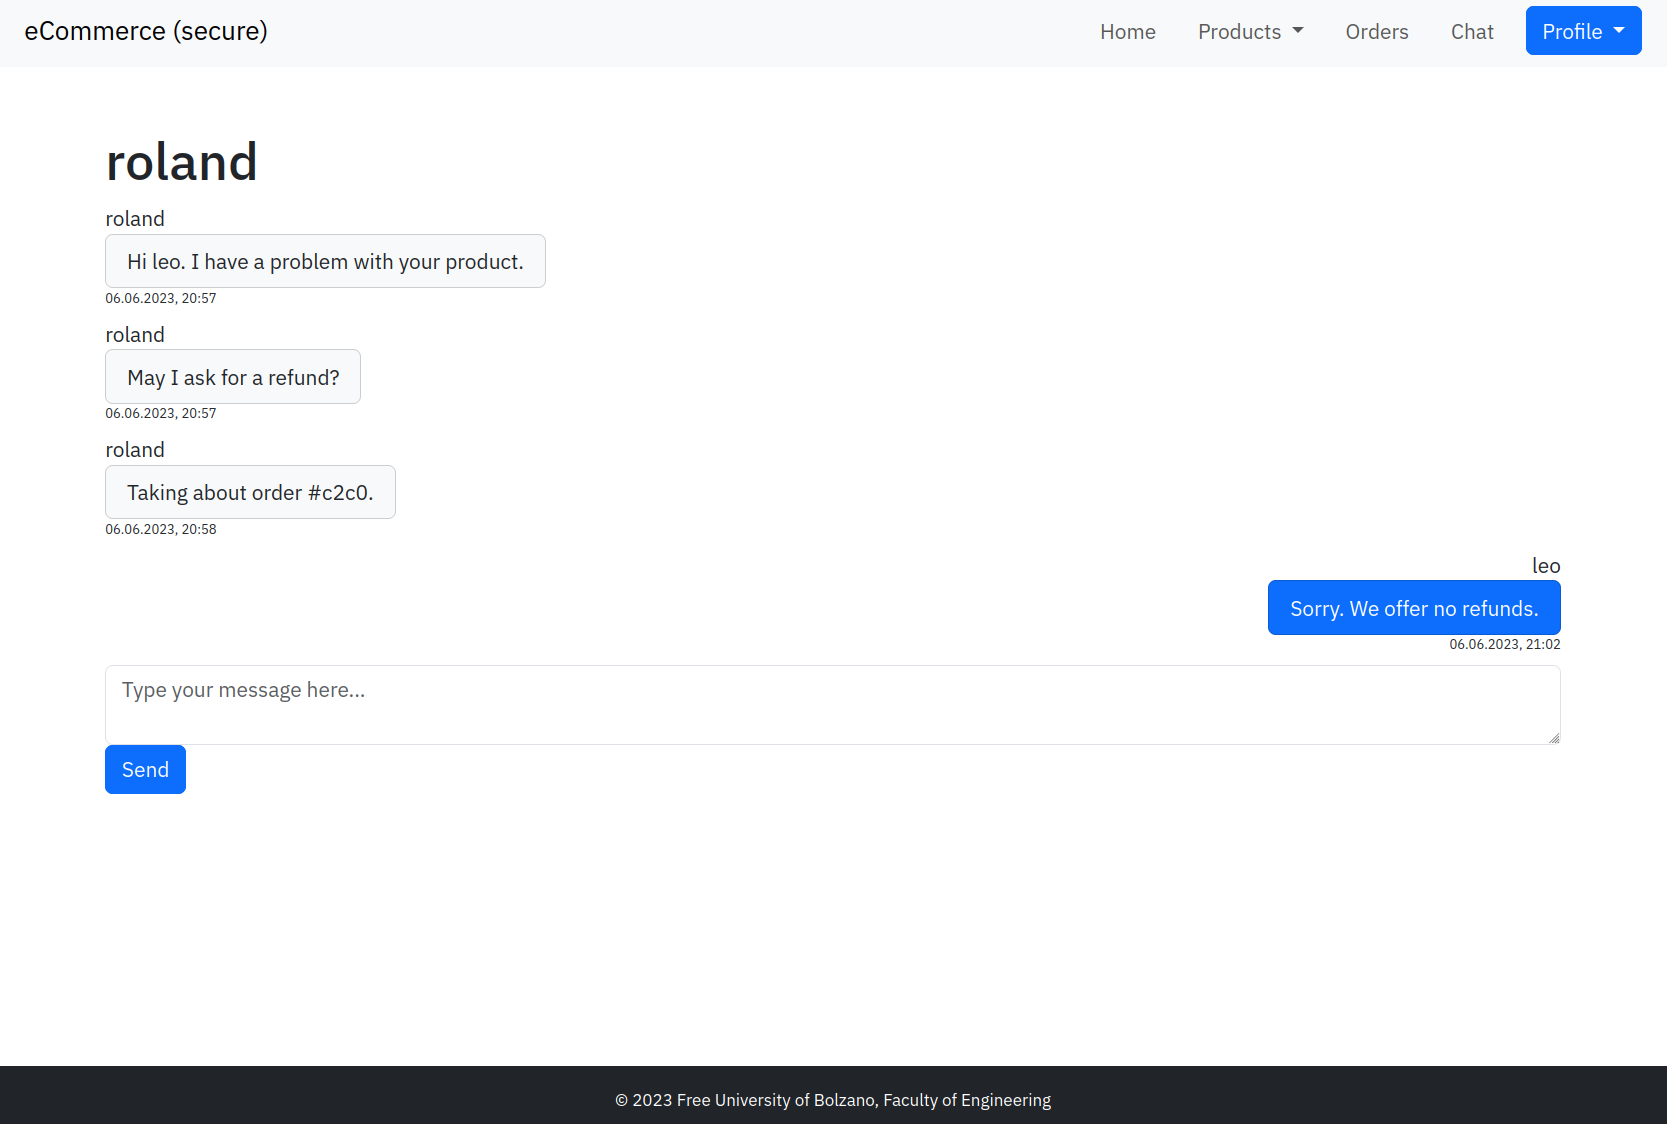
\includegraphics[width=\linewidth]{resources/chat.png}
        \caption{Un esempio di chat tra venditore e cliente.}
    \end{subfigure}
    \caption{Esempio di come i clienti possono chattare con i venditori.}
\end{figure}

L'applicazione offre ai clienti la possibilità di inviare messaggi ai venditori tramite una chat privata. I clienti possono cliccare sul nome del venditore sotto il nome del prodotto nella pagina delle informazioni sul prodotto. In questo modo si accede alla pagina della chat diretta con il fornitore selezionato. Tutte le chat avviate dal cliente sono disponibili anche nell'elenco delle chat, navigando con il pulsante "Chat" nell'intestazione della pagina web. Selezionando una delle chat, l'utente può digitare un messaggio nell'area di testo in fondo alla pagina e fare clic su "Submit" per inviarmi il messaggio. I messaggi sono memorizzati in modo criptato con l'algoritmo DES e non sono accessibili a nessuno, se non agli utenti che partecipano alla comunicazione.


\end{document}
